\documentclass[main.tex]{subfiles}
\begin{document}


\chapter{Folgen und Grenzwerte}


\section{Metrische Räume}

\begin{Definition}[Metrische Räume]
  Ein Paar $(X,d)$ ist ein \textbf{metrischer Raum}, wenn $X$ eine Menge ist und $d$ eine Distanzfunktion oder Metrik ist:\\
  $d: X \times X \to \R_{\geq 0}$, mit folgenden Eigenschaften
  \begin{itemize}
    \item Definitheit: $d(x,y) \geq 0, d(x,y) = 0 \Leftrightarrow x = y$
    \item Symmetrie: $d(x,y) = d(y,x)$
    \item Dreiecksungleichung: $d(x,y) + d(y,z) \geq d(x,z)$
  \end{itemize}
\end{Definition}

\begin{Beispiel}
  \begin{enumerate}
    \item $X \subseteq \R, d(x,y) = |x-y|$
    \item $X \subseteq \C = \R^2, d(x,y) = |x-y|$\\
      im Detail: $d(a + bi, c+di) = \sqrt{(a-c)^2+(b-d)^2}$\\
      Größte Schwierigkeit: Punkt 3 beweisen (Cauchy-Schwarz)
    \item Betrachte einen kombinatorischen zusammenhängenden Graphen $\mathcal{G}$. Sei $X$ die Menge aller Punkte von $\mathcal{G}$ und $d(x,y)$ der kürzeste Weges von $x$ nach $y$.
    \item Sei $X= \R^2$ Frankreich, mit Origo Paris. Bildhaft: Um mit dem Zug von a nach b zu kommen gibt es 2 Möglichkeiten, entweder b liegt auf dem Weg von a nach Paris, oder eben nicht. Im ersten Fall steigt man einfach vor Paris aus, im zweiten Fall muss man nach Paris, um dann umzusteigen.\\
      Das ist die SNCF-Metrik:
      $$d(x,y)=\left\{\begin{aligned}
        |x| + |y| & \text{ falls $x,y$ nicht kollinear}\\
        |x - y| & \text{ falls $x,y$ kollinear}
      \end{aligned}\right.$$
    \item Die Manhattan-Metrik: $\R^2 = X$, $d(x,y) = d({x_1 \choose x_2},{y_1 \choose y_2}) = |x_1 -y_1| + |x_2 - y_2|$
    \item $X = \mathcal{C}([a,b]) \qquad a \leq b \qquad f,g \in X$
      $$d(f,g) = \max(\{|f(x)-g(x)| \mid x \in [a,b]\})$$
      Die Definitheit und Symmetrie ergeben sich, die Dreiecksungleichung kann als Übung gemacht werden.
    \item Analog: $X = \mathcal{C}([a,b])$
      $$d(f,g) = \int_a^b |f(x)-g(x)| dx $$
      $$\tilde{d}(f,g) = \sqrt{\int_a^b (|f(x)-g(x)|)^2 dx }$$
  \end{enumerate}
\end{Beispiel}

\begin{Definition}[Ball]
  Sei $(X,d$) ein metrischer Raum, $x_0 \in X$, $r\geq 0$ reell. Wir nennen die Teilmenge
  $$B(x_0,r) = \{x \in X \mid d(x_0,x) < r \}$$
  offener Ball mit Zentrum $x_0$, Radius $r$.
\end{Definition}

\begin{Bemerkung}
  Für allgemeine Räume sind Radius und Zentrum nicht eindeutig bestimmt.
  \begin{Beispiel}
    $$X = \{x_0,x_1\} \qquad d(x_0,x_1) = 1$$
    $B(x_0,1) = B(x_1,2) = X$
  \end{Beispiel}
\end{Bemerkung}

\begin{Definition}[Beschränktheit]
  Sei $(X,d)$ ein metrischer Raum, $A \subseteq X$ eine Teilmenge. Wir sagen $A$ sei \textbf{beschränkt}, falls eine reelle Zahl $R \geq 0$ existiert mit $d(x,y) \leq R$ für $x,y \in A$.
\end{Definition}

\begin{Bemerkung}
  Ist $x_0 \in X$, so ist $A \subseteq X$ beschränkt $\Leftrightarrow \E R \geq 0$ mit $a \subseteq B(x_0,R)$.
\end{Bemerkung}

\begin{Definition}
  Sei $(X,d)$ ein metrischer Raum, $A \subseteq X$ eine Teilmenge. Wir sagen $A$ sei \textbf{offen} (in $X$), falls $\A x_0 \in A \E \delta > 0$ mit $B(x_0,\delta) \subseteq A$.

  Wir nennen $B \subseteq X$ abgeschlossen in $X$, falls $X \backslash B$ offen in $X$ ist.
\end{Definition}

\begin{Bemerkung}
  \begin{Theorem}
    Die Teilmengen $\emptyset,X$ von $X$ sind offen.\\
    Für $x_0 \in X, r> 0$ ist $B(x_0,r) \subseteq X$ offen.
  \end{Theorem}
  \begin{Beweis}
    Sei $x_1 \in B(x_0,r)$. Setze $\delta = r- d(x_0,x_1)$. Dann gilt $B(x_1 - \delta) \subseteq B(x_0,r)$.\\
    Sei $x\in B(x_1,\delta)$. Dann gilt:
    $$\begin{aligned}
        d(x,x_0) &\leq d(x,x_1) + d(x_1,x_0)\qquad\text{Dreiecksungleichung}\\
        &< \delta + d(x_1,x_0)\\
        &< r - (x_1,x_0) + d(x_1,x_0) = r
    \end{aligned}$$
    $\Rightarrow x \in B(x_0,r)$
  \end{Beweis}
\end{Bemerkung}

\begin{Theorem}
  Sei $(X,d)$ ein metrischer Raum.
  \begin{enumerate}
    \item Jede Vereinigung offener Teilmengen von $X$ ist offen.
    \item Jeder endlicher Durchschnitt offener Teilmengen von $X$ ist offen.
  \end{enumerate}
\end{Theorem}

\begin{Beweis}
  Sei $(U_i)_{i \in I}$ eine Familie offener Teilmengen von $X$.
  \begin{enumerate}
    \item Setze $U = \bigcup_{i \in I} U_i$. Zeige $U$ ist offen.\\
      Sei $x_0 \in U$. Dann existiert $i \in I$ mit $x_0 \in U_i$. $U_i$ ist offen $\Rightarrow \E \delta > 0$ mit $B(x_0,\delta) \subseteq U_i$.\\
      Also $B(x_0, \delta) \subseteq U_i \subseteq U$. $\Rightarrow U$ ist offen.
    \item Seien $U_1,U,2,..,U_n$ offene Teilmengen von $X$, setze $U = \bigcap_{i=1}^N U_i$. Sei $x_0 \in U$.\\
    Es gilt $x_0 \in U_i \A i \leq N$. Für jedes $i$ existiert $\delta_i > 0$ mit $B(x_0,\delta_i) \subseteq U_i$.\\
    Setze $\delta = min(\{\delta_1,...,\delta_N\} > 0$.\\
    Dann gilt $B(x_0,\delta) \subseteq B(x_0, \delta_i) \subseteq B(x_0,\delta_i) \subseteq U_i \A i$, also $B(x_0,\delta) \subseteq \bigcap_{i=1}^N U_i = U$
  \end{enumerate}
\end{Beweis}

\begin{Bemerkung}
  $A = (x_0 - \delta,x_0 + \delta) = B(x_0,\delta) \subseteq \R$ kann offen sein.\\
  Muss aber nicht als $A \subseteq \C$ offen sein!
\end{Bemerkung}


\subsection{Stetigkeit in metrischen Räumen}

\begin{Definition}[Stetigkeit]
  Seien $(X,dX),(Y,dY)$ metrische Räumen und $f: X \to Y$.
  \begin{itemize}
    \item  Wir sagen $f$ sei \textbf{stetig} falls
      $$\A \varepsilon > 0 \E \delta > 0 :d_X (x_1,x_2) < \delta \Rightarrow d_Y(f(x_1),f(x_2))<\varepsilon \A x \in X$$
      $f$ ist stetig (auf $X$) falls $f$ in jedem Punkt $x_0 \in X$ stetig ist.\\
      Ist $x \subseteq \R$ und $Y = \R$ mit der Standardmetirk ..., so erhalten wir den bekannten Stetigkeitsbegriff.
    \item Wir sagen $f$ sei \textbf{gleichmäßig stetig} falls
      $$\A \varepsilon > 0 \E \delta > 0 :d_X (x_1,x_2) < \delta \Rightarrow d_Y(f(x_1),f(x_2))<\varepsilon \A x_1,x_2 \in X$$
    \item Wir sagen $f$ sei \textbf{Lipschitz-stetig} falls
      $$\E L \geq 0 : d_Y(f(x_1),f(x_2)) < L*d_X (x_1,x_2)$$
      $L$ ist die Lipschitzkonstate für $f$
  \end{itemize}
\end{Definition}

\begin{Definition}[Isometrie]
  Wir nennen $f:X\to Y$ \textbf{Isometrie} falls
  $$d_Y(f(x_1),f(x_2)) = d_X (x_1,x_2) \A x_1,x_2 \in X$$
\end{Definition}

\begin{Theorem}
  \begin{center}
    Isometrie $\Rightarrow$ Lipschitz $\Rightarrow$ ...
  \end{center}
\end{Theorem}

\begin{Theorem}
  Seien $(X,d)$ und $(Y,d)$ metrische Räume und $f:X \to Y$. Dann sind äquivalent:
  \begin{enumerate}
    \item $f$ ist stetig.
    \item $\A U \subseteq Y$ mit $U$ offen ist $f^{-1} \subseteq X$ offen.
  \end{enumerate}
\end{Theorem}

\begin{Beweis}
  Die Funktion $f$ ist stetig falls (per Definition)
  $$\A x_0 \in X, \A \varepsilon > 0 \E \delta >0 : d(x,x_0)<\delta \Rightarrow d(f(x),f(x_0)) < \varepsilon \A x \in X$$
  Das heißt: $f(B(x_0,\delta)) \subseteq B(f(x_0),\varepsilon)$
  \begin{itemize}
    \item $1 \Rightarrow 2$:\\
      Sei $f$ stetig, $U \subseteq Y$ offen. Zu zeigen: $f^{-1}(U) \subseteq X$ offen. Sei $x_0 \in f^{-1}(U)$, also $f(x_0) \in U$.\\
      $U$ ist offen $\Rightarrow \E \varepsilon > 0$ mit $B(f(x_0),\varepsilon) \subseteq U$.\\
      $f$ stetig $\Rightarrow \E \delta > 0$ mit $f(B(x_0,\delta)) \subseteq B(f(x_0),\epsilon) \subseteq U$\\
      also
      $$B(x_0,\delta) \subseteq f^{-1}(U) \Rightarrow f^{-1} \text{ offen}$$
    \item $2 \Rightarrow 1$:\\
      Sei $x_0 \in X, \varepsilon > 0$. Betrachte $B(f(x_0),\varepsilon) \subseteq Y$ (ist bewiesenermaßen offen). Also ist das Urbild $f^{-1}(B(f(x_0),\varepsilon) \subseteq X$ ebenfalls offen und enthält notwendigerweise $x_0$. Das bedeutet, es existiert also ein $\delta > 0$ mit $B(x_0,\delta) \subseteq f^{-1}(B(f(x_0),\varepsilon) \subseteq X$.\\
      Folgt $f(B(x_0,\delta)) \subseteq B(f(x_0),\varepsilon)$. Also ist $f$ stetig.
  \end{itemize}
\end{Beweis}


\section{Folgen}

\begin{Definition}[Folge]
  Sei $X$ eine Menge. Eine \textbf{Folge} in $X$ ist eine Funktion $$x: \N \to X$$.
  Schreibweise: \begin{itemize}
    \item Wir schreiben $x_n$ für $x(n) \epsilon$ für $n \in \N$.
    \item Wir schreiben $(x_n)_{n=0}^\infty$ für die Funktion $x$.
    \item Wir sagen $(x_n)_{n=0}^\infty$ sei \textbf{konstant} falls $x$ eine konstante Funktion ist.
    \item Das Bild der Folge $(x_n)_{n=0}^\infty$ ist $x(\N) = \{x_n \mid n \in \N\} \subseteq X$
  \end{itemize}
\end{Definition}

\begin{Definition}[Grenzwert]
  Es sei $(X,d)$ ein metrischer Raum und sei $(x_n)_{n=0}^\infty$ eine Folge in $X$.

  Ein Element $a \in X$ heißt \textbf{Grenzwert} oder \textbf{Limes} von $(x_n)$ falls
  $$\A \varepsilon : \E N \in \N \text{ mit } n \geq N \Rightarrow d(x_n,a) < \varepsilon$$
\end{Definition}

\begin{Beispiel}
  \begin{itemize}
    \item $X = \R$, $d(x,y)= |x-y|$. Betrachte $(x_n)_{n=0}^\infty$ mit $x_n = n$.

      Diese Folge hat keinen Grenzwert. $\A a \in \R$ ist $a$ nicht ein Grenzwert der Folge.
      \begin{Beweis}
        Sei $a \in \R$. Angenommen $a$ sei ein Grenzwert, dann existiert ein $N \in \N$ mit $\A n \geq N : d(a,x_n) = |a-x_n| < \varepsilon = \dfrac{1}{2}$

        Insbesondere ist $|a-x_n| < \dfrac{1}{2}$ und $|a-(N+1)| < \dfrac{1}{2}$. Das widerspricht der Dreiecksungleichung.
      \end{Beweis}
    \item $(x_n)_{n=0}^\infty$ mit $x_n = \dfrac{(-1)^n}{n!} \left(= 1,-1,\dfrac{1}{2},-\dfrac{1}{6},...\right)$

      Diese Folge hat genau einen Grenzwert $a = 0$.
    \item $X = \mathcal{C}([0,1])$ (die Menge aller Stetigen Funktionen auf diesem Intervall), $d(f,g) = \int_0^1 |f-g| dx$.

      Betrachte die Folge $(f_n)_{n=0}^\infty$ gegeben durch $c_n = \dfrac{1}{n+2}$. Diese Folge hat einen Grenzwert: $g = (konstant = 1) = 1_{[0,1]}$.
      \begin{Beweis}
        $$d(f_n,g) = \int_0^1 |f_n - g|dx = \int_0^1 \left|\dfrac{1 - n - 2}{n-2}\right| dx = \dfrac{1}{n+2}$$
        Dieser Wert ist laut archimedischem Prinzip kleiner als jeder beliebiger Positiver Wert, also ist $g$ ein Grenzwert.
      \end{Beweis}
      Aber ist dieser Grenzwert der einzige?
  \end{itemize}
\end{Beispiel}

\begin{Theorem}
  Sei $(X,d)$ ein metrischer Raum, $(x_n)_{n=0}^\infty$ eine Folge in $X$. Sind $a,b \in X$ Grenzwerte dieser Folge, so gilt $a = b$.
\end{Theorem}

\begin{Beweis}
  Sei $\varepsilon > 0$. $a$ ist Grenzwert $\Rightarrow \E N$ mit $n\geq N \Rightarrow d(x_n,a) < \dfrac{\varepsilon}{2}$\\
  $b$ ist Grenzwert $\Rightarrow \E M$ mit $n\geq M \Rightarrow d(x_n,b) < \dfrac{\varepsilon}{2}$\\
  Für $n \geq \max(\{N,M\})$ gilt dann: $d(a,b) \leq d(x_n,a) + d(x_n,b) < \varepsilon$\\
  Daraus folgt, dass $d(a,b) = 0 \Rightarrow a = b$
\end{Beweis}

\begin{Definition}
  Eine Folge $(x_n)_{n=0}^\infty$ heißt
  \begin{itemize}
    \item konvergent, falls ein Grenzwert $a \in X$ für diese Folge existiert. Wir schreiben:
        $$a = \lim \limits_{n \to \infty} x_n$$
    \item beschränkt, wenn ihr Bild $\{x_n \mid n \in \N\}\subseteq X$ beschränkt ist.
  \end{itemize}
\end{Definition}

\begin{Theorem}
  Sei $(x_n)_{n=0}^\infty$ eine Folge in $(X,d)$. Ist die Folge konvergent, so ist sie beschränkt.
\end{Theorem}

\begin{Beweis}
  Wir zeigen $\E R \geq 0$ mit $x_n \in B(x_0,R)$ für alle $n \in \N$. Setze $a = \lim \limits_{n \to \infty} x_n$. Dann existiert ein $N \in \N$ mit $d(x_n,a) < 1$ (frei gewählt).\\
  Sei $R \in \R$ mit $R\geq d(x_0,x_n)$ für $0 \leq n < N$ und $R \geq d(x_0,a)+1$.

  Jetzt gilt: $x_n \in B(x_0,R)$ für $0 \leq n < N$ und für $n \geq N$ gilt:
  $$d(x_0,x_n) \leq d(x_0,a) + d(a,x_n) < d(x_0,a)+ 1 \leq R$$
  Also $x_n \in B(x_0,R)$
\end{Beweis}

\begin{Definition}[Häufungspunkt]
  Sei $(X,d)$ ein metrischer Raum, $(x_n)_{n=0}^\infty$ eine Folge in $X$. Ein Element $a \in X$ heißt \textbf{Häufungspunkt} der Folge falls
  $$\A \varepsilon > 0 : \A N \in \N: \E n \in \N : d(x_n,a) < \varepsilon$$
\end{Definition}

\begin{Beispiel}
  $X = \C$, setze $x_n = i^n + \dfrac{1}{2^n}$. (ohne den Bruch wäre das 1, i, -1, -i, 1...)

  Die Punkte $\{1,i,-1,-i\}$ sind alle Häufungspunkte der Folge.
\end{Beispiel}

\begin{Bemerkung}[Warnung]
  Häufungspunkte einer Folge sind im Allgemeinen nicht dasselbe wie Häufungspunkte des Bildes $\{x_n \mid n \in \N\}$
\end{Bemerkung}

\begin{Beispiel}
  $X = [0,1]$ und $d$ die Standardmetrik. Sei $x_n = n \sqrt{2} - \lfloor n \sqrt{2} \rfloor$.
  \begin{Theorem}
    Jedes Element $a \in [0,1]$ ist ein Häufungspunkt dieser Folge.
  \end{Theorem}
\end{Beispiel}

\begin{Theorem}
  Sei $(x_n)_{n=0}^\infty$ eine konvergierende Folge in $(X,d)$ mit Grenzwert $a \in X$.

  Dann ist $a$ der einzige Häufungspunkt dieser Folge.
\end{Theorem}

\begin{Beweis}
  Aus den Definitionen folgt: $a$ ist ein Häufungspunkt der Folge. Sei $b \in X$ ein Häufungspunkt von $(x_n)_{n=0}^\infty$. Sei $\varepsilon > 0$.

  $$\E N \in \N : d(a,x_n) < \dfrac{\varepsilon}{2} \A n \geq N$$
  Da $b$ ein Häufungspunkt ist, gilt: $\E m \geq N : d(x_m,b) < \dfrac{\varepsilon}{2}$. Jetzt folgt
  $$\begin{aligned}
    d(a,b) &\leq d(a,x_m) + d(x_m,b)\\
    &\leq \dfrac{\varepsilon}{2} + \dfrac{\varepsilon}{2} = \varepsilon
  \end{aligned}$$
  $\Rightarrow d(a,b) = 0 \Rightarrow a = b$
\end{Beweis}

\begin{Definition}[Teilfolge]
  Sei $(x_n)_{n=0}^\infty$ eine Folge in einer Menge $X$. (Die Metrik spielt hier keine Rolle). Eine Folge $(y_k)_{k=0}^\infty$ in $X$ heißt \textbf{Teilfolge} von $(x_n)_{n=0}^\infty$ falls eine streng monoton steigende Funktion $f:\N \to \N$ existiert, mit
  $$y_k = x_{f(k)} \A k \in \N$$
\end{Definition}

\begin{Beispiel}
  $$y_k = x_{2k}: x_0,x_2,x_4,...$$
\end{Beispiel}

\begin{Theorem}
  Seien $(x_n)_{n=0}^\infty$ eine Folge in $(X,d)$, $a \in X$. Sind äquivalent:
  \begin{enumerate}
    \item $a$ ist ein Häufungspunkt von $(x_n)_{n=0}^\infty$
    \item Es existiert eine konvergierende Teilfolge $(y_k)_{k=0}^\infty$ von $(x_n)_{n=0}^\infty$ mit Grenzwert $a$
  \end{enumerate}
\end{Theorem}

\begin{Beweis}
  \begin{itemize}
    \item $1) \Rightarrow 2)$\\
      Angenommen $a \in X$ ist Häufungspunkt. Also existiert ein $n_0 \in \N$ mit $d(a,x_0) \leq 1$.

      Es existiert ein $n_1 \in \N$ mit $n_1 \geq n_0 + 1$ und $d(a,x_{n_1}) < \frac{1}{2}$.

      Es existiert ein $n_2 \in \N$ mit $n_2 \geq n_1 + 1$ und $d(a,x_{n_2}) < \frac{1}{4}$.

      Es existiert ein $n_3 \in \N$ mit $n_3 \geq n_2 + 1$ und $d(a,x_{n_3}) < \frac{1}{8}$.

      ... (induktiv)

      Es existiert ein $n_k \in \N$ mit $n_k \geq n_{k-1} + 1$ und $d(a,x_{n_k}) < \dfrac{1}{2^k}$.

      Wir konstruieren jetzt rekursiv die Folge $(y_k)_{k=0}^\infty$ mit $y_k = x_{n_k}$. Dies ist eine Teilfolge von $(x_n)_{n=0}^\infty$ mit $d(y_k,a) < 2^{-k}$. Die Folge $(y_k)_{k=0}^\infty$konvergiert mit Grenzwert $a$.
    \item $2) \Rightarrow 1)$

      Sei $(y_k)_{k=0}^\infty$ eine konvergierende Teilfolge mit Grenzwert $a$. Sei $\varepsilon > 0$, $N \in \N$. Setze $y_k = x_{f(k)}$ für $f:\N \to \N$ streng monoton.

      Da $f$ streng monoton ist, gilt insbesondere $f(k) \geq k \A q \in \N$ und
      $$\E K \in \N : k \geq K \Rightarrow d(y_k, a) < \varepsilon$$

      Wähle $k \in \N$ mit $k \geq K$ und $k \geq N$ und setze $n = f(k)$. Dann gilt $n \geq N$ und $D(a,x_n) = d(a,y_k) \leq \varepsilon$
  \end{itemize}
\end{Beweis}

\begin{Theorem}
  Es seien $(X,d)$ und $(Y,d)$ metrische Räume, $f: X \to Y$. Sind äquivalent:
  \begin{enumerate}
    \item $f$ ist stetig
    \item Ist $(x_n)_{n=0}^\infty$  eine konvergente Folge in $X$ mit Grenzwert $a \in X$ so ist $(f(x_n))_{n = 0}^\infty$ konvergent mit Grenzwert $f(a)$.
  \end{enumerate}
\end{Theorem}

\begin{Bemerkung}
  \begin{itemize}
    \item Dieses Theorem wir im Allgemeinen \textbf{nicht} zum Beweis der Stetigkeit benutzt.
    \item Es kann allerdings als Gegenbeweis verwendet werden, da es genügt, ein Gegenbeispiel zu finden.
    \item Wir werden es vor Allem zur Berechnung von Grenzwerten verwenden.
  \end{itemize}
\end{Bemerkung}

\begin{Beweis}
  \begin{itemize}
    \item $1) \Rightarrow 2)$\\
      Sei $f$ stetig, $(x_n)_{n=0}^\infty$ konvergent, Grenzwert $a \in X$. Sei $\varepsilon > 0$\\
      $f$ ist stetig bei $a$: $\E \delta > 0 : d(x,a) <  \delta \Rightarrow d(f(x),f(a)) < \varepsilon$ * \\
      $(x_n)_{n=0}^\infty$ kovergiert gegen $a$: $\E N \in \N$ mit $n \geq N \Rightarrow d(x_n,a) < \delta$ **\\
      Für $n \geq N$ gilt also wegen * und ** $d(f(x_n),f(a)) < \varepsilon$.\\
      $\Rightarrow f(a)$ ist Grenzwert der Folge $(f(x_n))_{n = 0}^\infty$.
    \item $\lnot 1) \Rightarrow \lnot 2)$\\
      Angenommen $f$ sei nicht stetig in einem Punkt $a \in X$. Also
      $$ \E \varepsilon > 0 : \A \delta >0: \E x \in X : d(a,x) < \delta \text{ und } d(f(a),f(x)) > \varepsilon$$
      Wir wählen wür jedes $n \in \N$ ein $x_n \in X$ mit $d(x_n,a) < 2^{-n}$ und $d(f(x_n),f(a)) > \varepsilon$.\\
      Die Folge $(x_n)_{n=0}^\infty$ in $X$ konvergiert gegen $a$.\\
      Die Folge $(f(x_n))_{n = 0}^\infty$ konvergiert \textbf{nicht} gegen $f(a)$ (denn die Distanz zu $f(a)$ ist immer größer als $\varepsilon$)
  \end{itemize}
\end{Beweis}

\subsection{Cauchy-Folgen}

\begin{Definition}[Cauchy-Folgen]
  Sei $(X,d)$ ein metrischer Raum und $(x_n)_{n=0}^\infty$ eine Folge in $X$. Wir nennen $(x_n)_{n=0}^\infty$ eine \textbf{Cauchy-Folge}, falls
  $$\A \varepsilon > 0 :  \E N \in \N : d(x_n,x_m) < \varepsilon \A n,m \geq N$$
  \begin{Bemerkung}
    Es wird nicht nach einem Grenzwert verlangt.
  \end{Bemerkung}
\end{Definition}

\begin{Theorem}
  Jede konvergente Folge ist eine Cauchy-Folge.
\end{Theorem}

\begin{Beweis}
  Sei $(x_n)_{n=0}^\infty$ konvergent mit Grenzwert $a \in X$. Sei $\varepsilon > 0$, dann existiert $N \in \N$ mit $d(a,x_n) < \dfrac{\varepsilon}{2} \A n \geq N$.\\
  Also gilt für alle $n,m \geq N$
  $$\begin{aligned}
    d(x_n,x_m) &\leq d(x_n,a) + d(a,x_m)\\
    &\leq \dfrac{\varepsilon}{2} + \dfrac{\varepsilon}{2} = \varepsilon
  \end{aligned}$$
\end{Beweis}
\begin{Bemerkung}
  Im Allgemeinen gilt: nicht jede Cauchy-Folge konvergiert.
  \begin{Beispiel}
    Betrachten wir $X = (0,1)$ mit $d$ üblich: $d(x,y) = |x-y|$ und die Folge $x_n = 10^{-n}$.\\
    Diese Folge konvergiert \textbf{nicht} (denn $0 \notin X$) aber ist eine Cauchy-Folge.
  \end{Beispiel}
  \begin{Beispiel}
    Definiere: $F_0 = 0, F_1 = 1$ und rekursiv: $F_n = F_{n-1} + F_{n-2}$, die Fibonacci-Folge.\\
    Ebenfalls definiere eine Folge $(x_n)_{n=0}^\infty$ in $\Q$ durch $x_n = \dfrac{F_n}{F_n+1}$. Diese konvergiert nicht, ist jedoch eine Cauchy-Folge.\\
    In $\R$ konvergiert dieselbe Folge gegen $a = \Phi = \dfrac{\sqrt{5}-1}{2}=1,6...$
  \end{Beispiel}
\end{Bemerkung}

\begin{Definition}[Vollständigkeit]
  Ein metrischer Raum $(X,d)$ heißt \textbf{vollständig} falls jede Cauchy-Folge in $X$ konvergiert.
\end{Definition}
\begin{Beispiel}
  \begin{itemize}
    \item Aus den vorherigen Beispielen folgt: $X = (0,1)$ und $X = \Q$ sind nicht vollständig.
      \begin{Bemerkung}
        Es ist üblich, $\R$ als die Vervollständigung von $\Q$ zu konstruieren.
      \end{Bemerkung}
    \item Die Räume $\R,\C$ sind vollständig (wird allerdings später behandelt)
  \end{itemize}
\end{Beispiel}

\begin{Theorem}[Banach'scher Fixpunktsatz]
  Sei $(X,d)$ ein nichtleerer, vollständiger metrischer Raum, und sei $T : X \to X$ eine Abbildung mit der Eigenschaft
  $$\A 0 \leq \lambda \leq 1 : d(T(x),T(y)) \leq d(x,y)* \lambda$$
  \begin{Bemerkung}
    Das bedeutet dass diese Abbildung Lipschitz-stetig sein muss mit einer Lipschitzkonstante, die kleiner als 1 ist.
  \end{Bemerkung}
  Dann existiert ein eindeutiges $a \in X$ mit $T(a) = a$
\end{Theorem}

\begin{Bemerkung}
  Dient beispielsweise bei der Lösung von Differentialgleichungen der Bestimmung einer eindeutigen Lösung.
\end{Bemerkung}

\begin{Beweis}
  \begin{itemize}
    \item Eindeutigkeit:\\
      Gilt $T(a) = a$ und $T(b) = b$, so gilt:
      $$d(a,b) = d(T(a),T(b)) \leq d(a,b) * \lambda \Rightarrow d(a,b) = 0 \Rightarrow a = b$$
    \item Existenz:\\
      Wähle $x_0 \in X$ und betrachte die Folge $x_0,x_1 = T(x_0),..,x_n =T(x_{n-1})$.\\
      Behauptung:
      \begin{enumerate}
        \item Diese Folge ist eine Cauchy-Folge, also konvergiert sie da $X$ vollständig ist.
        \item Für $a = \lim \limits_{n \to \infty} x_n$ gilt $T(a) = a$
      \end{enumerate}
      \begin{enumerate}
        \item Sei $\varepsilon > 0$. Betrachte zu $n \in \N$:
          $$\begin{aligned}
            d(x_n,x_{n+1}) &\leq d(x_{n-1},x_n)*\lambda \leq d(x_{n-2},x_{n-1})*\lambda^2 \leq ...\\
            &\leq d(x_0,x_1)*\lambda^n
          \end{aligned}$$
          Denn $x_n = T(x_{n-1})$ und der Faktor zwischen den Distanzen per Definition.\\
          Für $N \in \N$ ...
      \end{enumerate}
  \end{itemize}
  Ein eleganterer Beweis ist später aufgeführt.
\end{Beweis}



\section{Folgen reeller und komplexer Zahlen}
Es handelt sich hier um Spezialfälle eines metrischen Raums. Zur Distanz können wir jetzt + und * verwenden und Ungleichungen aufstellen. Dies erlaubt uns detaillierte Aussagen.

Zusätzlich zur Metrik $d$ auf $\R$ ($d(x,y) = |x-y|$) haben wir $(+,*,\leq)$. Wir können von nun an Folgen $(x_n)_{n=0}^\infty$ und $(y_n)_{n=0}^\infty$ in $\R$ addieren und multiplizieren:

\begin{Theorem}
  \begin{itemize}
    \item $(x_n)_{n=0}^\infty + (y_n)_{n=0}^\infty = (x_n + y_n)_{n=0}^\infty$
    \item $(x_n)_{n=0}^\infty * (y_n)_{n=0}^\infty = (x_n * y_n)_{n=0}^\infty$
    \item $\alpha * (x_n)_{n=0}^\infty = (\alpha * x_n)_{n=0}^\infty$ mit $\alpha \in \R$
  \end{itemize}
\end{Theorem}

\begin{Theorem}
  Seien $(x_n)_{n=0}^\infty$ und $(y_n)_{n=0}^\infty$ konvergente Folgen in $\R$. Dann gilt:
  \begin{enumerate}
    \item $(x_n + y_n)_{n=0}^\infty$ konvergiert und es gilt:\\
      $\lim \limits_{n \to \infty} (x_n + y_n) = \lim \limits_{n \to \infty} (x_n) + \lim \limits_{n \to \infty} (y_n)$
    \item $(x_n * y_n)_{n=0}^\infty$ konvergiert und es gilt:\\
      $\lim \limits_{n \to \infty} (x_n * y_n) = \lim \limits_{n \to \infty} (x_n) * \lim \limits_{n \to \infty} (y_n)$
    \item Angenommen $x_n \neq 0 \A n$ und $\lim \limits_{n \to \infty} (x_n)_{n=0}^\infty \neq 0$. Dann konvergiert $(x_n^{-1})_{n=0}^\infty$ und es gilt:\\
      $\lim \limits_{n\to \infty} (x_n^{-1}) = \lim \limits_{n\to \infty} (x_n)^{-1}$
  \end{enumerate}
\end{Theorem}

\begin{Beweis}
  \begin{enumerate}
    \item Setze $a = \lim \limits_{n \to \infty} x_n$ und $b = \limn y_n$. Sei $\varepsilon >0$. Es existiert ein $N \in \N$ mit:\\
      $|x_n - a|< \dfrac{\varepsilon}{2}$ und $|y_n - b|< \dfrac{\varepsilon}{2}$ für alle $n \geq N$\\
      Dann gilt für $n\geq N$ auch:
      $$|(x_n+y_n) - (a+b)| = |x_n -a + y_n -b| \leq |x_n -a| + |y_n -b| \leq \dfrac{\varepsilon}{2} + \dfrac{\varepsilon}{2} = \varepsilon$$\\
      Oder:\\
      Die Abbildung $s:\R \times \R \to \R$, $s(x,y) = x+y$ ist stetig, und die Folge $(x_n , y_n)_{n=0}^\infty$ in $\R^2$ konvergiert gegen $(a,b)$.\\
      Folgenkriterium für Stetigkeit: Die Folge $s(x_n , y_n)_{n=0}^\infty = (x_n + y_n)_{n=0}^\infty$ konvergiert ebenfalls, mit Grenzwert $s(a,b)=a+b$
    \item Die Abbildung $m: \R \times \R \to \R$ gegeben durch $m(x,y) = xy$ ist stetig. Es folgt die selbe Überlegung wie in 1.
    \item Die Abbildung $i: \R\backslash\{0\} \to \R$ mit $i(x) = x^{-1}$ ist stetig.
  \end{enumerate}
\end{Beweis}

\begin{Korollar}
  Die Menge aller konvergenten Folgen in $\R$ bildet einen Vektorraum bezüglich der gegebenen Addition und Skalarmultiplikation.\\
  Die Abbildung $\{$Konvergente Folgen in $\R\} \to \R$ mit $(x_n)_{n=0}^\infty \mapsto \lim \limits_{n \to \infty} (x_n)$ ist wohldefiniert und linear.
\end{Korollar}

\begin{Theorem}
  Seien $(x_n)_{n=0}^\infty$ und $(y_n)_{n=0}^\infty$ konvergierende Folgen in $\R$ mit Grenzwerten $a = \lim x_n$ und $b = \lim y_n$.
  \begin{enumerate}
    \item Gilt $a < b$, so existiert ein $N \in \N$ mit
      $$x_n < y_n \A n \geq N$$
      \begin{Bemerkung}
        Die Umkehrung dieser Aussage gilt \textbf{nicht}. Es kann sein, dass alle Werte einer Folge immer echt kleiner als die Werte der anderen sind, aber dass die Grenzwerte beider Folgen gleich sind.
      \end{Bemerkung}
    \item Existiert ein $N \in \N$, so dass $x_n \leq y_n$ für $n \geq N$ so gilt $a \leq b$.
  \end{enumerate}
\end{Theorem}
\begin{Beweis}
  \begin{enumerate}
    \item Setze $\varepsilon = \dfrac{b-a}{3} > 0$. Es existiert ein $N \in \N$ mit
      $$|x_n - a| < \varepsilon \text{ und } |y_n - b| < \varepsilon \A n \geq N$$
      $\Rightarrow x_n \leq y_n$ Siehe Foto
    \item Das ist die Negation von (1).
  \end{enumerate}
\end{Beweis}

\begin{Lemma}[Sandwich-Kriterium]
  Es seien $(x_n)_{n=0}^\infty$ und $(y_n)_{n=0}^\infty$ und $(z_n)_{n=0}^\infty$ Folgen in $\R$. Angenommen:
  \begin{itemize}
    \item $x_n \leq y_n \leq z_n \A n (n \geq N)$
    \item $\limn x_n = \limn z_n = a \in \R$
  \end{itemize}
  Dann konvergiert $(y_n)_{n=0}^\infty$ mit $\lim y_n = a$
\end{Lemma}
... oder auch als das Sammich-Kriterium bekannt (c.f Urbandictionnary).

\begin{Beweis}
  Sei $\varepsilon > 0$. $\E N \in \N$ mit
  $$|x_n - a| < \varepsilon \text{ und } |z_n - a| < \varepsilon \A n \geq N$$
  Dann gilt auch $|y_n - a| < \varepsilon$ weil $x_n \leq y_n \leq z_n$ nach umgekehrter Dreiecksungleichung.\\
  Siehe Foto.
\end{Beweis}

\begin{Beispiel}
  Betrachte die Folge $(x_n)_{n=0}^\infty$ mit $x_0 = 1$ und $x_n = \sqrt[n]{n}$ für $n \geq 1$.\\
  Behauptung: Diese Folge konvergiert gegen 1.\\
  Definiere $y_n = x_n -1 \geq 0$\\
  Trick: $$n = (1+y_n)^n = \sum \limits_{k=0}^n {n \choose k} y_n^k \geq {n \choose 2} y_n^2 = \dfrac{n(n-1)}{2}y_n^2$$
  $\Rightarrow 0 \leq y_n \leq \sqrt{\dfrac{2}{n-1}} := z_n$ für $n\geq 2$.\\
  Jetzt gilt: $\limn 0 = 0$, $\limn z_n = 0$ $\Rightarrow \limn y_n = 0$. Dies muss für $z_n$ mit dem archimedischen Prinzip und der Stetigkeit der Wurzelfunktion definiert werden. ($x^2$ ist stetig und monoton also ist $\sqrt{x}$ stetig also ist $\lim y_n = \lim \sqrt{\dfrac{2}{n-1}}$.)
\end{Beispiel}

\begin{Definition}
  Eine Folge $(x_n)_{n=0}^\infty$ in $\R$ heißt monoton steigend, falls $x_n \leq x_m$ für alle $n \leq m$ in $\N$\\
  Bei strengen Ordnunungsrelationen sprechen wir von strenger Monotonie.\\
  Analog für fallend.
\end{Definition}
\begin{Bemerkung}
  Spezialfall der Definition der Monotonie für Funktionen.
\end{Bemerkung}

\begin{Theorem}
  Sie $(x_n)_{n=0}^\infty$ eine monotone und beschränkte Folge. Dann konvergiert diese Folge.
\end{Theorem}
\begin{Beweis}
  Setze $a = sup\{x_n \mid n \in \N\}$. Angenommen $(x_n)_{n=0}^\infty$ sei monoton steigend. (oder anders herum falls wir nach inf suchen).

  Sei $\varepsilon > 0$. Dann $\E N \in \N$ mit $|x_N - a|< \varepsilon$ und außerdem $x_n \leq a$. Für alle $n \geq N$ gilt dann $x_N \leq x_n \leq a$ (erste Ungleichung wegen Monotonie, 2. wegen Definition von sup)\\
  Also $|x_n - a| < \varepsilon$ für alle $n \geq N$
\end{Beweis}

\begin{Definition}[Limsup]
  Sei $(x_n)_{n=0}^\infty$ eine beschränkte Folge in $\R$. Für $k \in \N$ setze
  $$s_k = \sup(\{ x_n \mid n \geq k\})$$
  Wir definieren:
  $$\limsup_{n\to \infty} x_n := \lim \limits_{k \to \infty} s_k$$
  Analog:
  $$t_k = \inf(\{ x_n \mid n \geq k\})$$
  Wir definieren:
  $$\liminf_{n\to \infty} x_n := \lim \limits_{k \to \infty} t_k$$
\end{Definition}

\begin{Beispiel}
  Betrachte die Folge $(x_n)_{n=1}^\infty$ gegeben durch $x_n = (-1)^n + \dfrac{1}{n}$.

  \begin{center}
    \begin{tikzpicture}
    \begin{axis}[
      domain=0:20,
      axis x line = center,
      axis y line = center,
      xlabel={$n$},
      ylabel={$x_n$},
      ]
      \addplot [samples at={0,...,20},only marks] {(-1)^x + 1/x};
      \end{axis}
    \end{tikzpicture}
  \end{center}
  Für die einzelnen Werte ist also:
  $$\begin{array}{c|c c c c c c c}
    n & 1 & 2 & 3 & 4 & 5 & 6 & ... \\
    \hline
    x_n & 0 & 1+\dfrac{1}{2} & -1+\dfrac{1}{3} & 1+\dfrac{1}{4} & -1+\dfrac{1}{5} & 1+\dfrac{1}{6} & ... \\
    \\
    s_n & 1+\dfrac{1}{2} & 1+\dfrac{1}{2} & 1+\dfrac{1}{4} & 1+\dfrac{1}{4} & 1+\dfrac{1}{6} & 1+\dfrac{1}{6} & ... \\
    \\
    t_n & -1 & -1 & -1 & -1 & -1 & -1 & ... \\
  \end{array}$$
  Es folgt:
  $$\limsup x_n = \lim s_n = 1 \quad \liminf x_n = \lim t_n = -1$$
\end{Beispiel}

\begin{Theorem}
  Sei $(x_n)_{n=0}^\infty$ eine beschränkte Folge in $\R$, mit $a = \limsup_{n\to \infty} x_n$.\\
  Dann gilt für alle $\varepsilon > 0$:
  \begin{itemize}
    \item $\{n \mid x_n > a + \varepsilon \}$ ist endlich
    \item $\{n \mid x_n > a - \varepsilon \}$ ist unendlich
  \end{itemize}
\end{Theorem}

\begin{Beweis}
  \item Sei $\varepsilon > 0$, setze $s_n = \sup (\{ x_k \mid k \geq n \})$ für $n \in \N$. Diese Folge ist monoton fallend und konvergiert gegen $a$. Es existiert ein $N \in \N$ mit
    $$a \leq s_N < a + \varepsilon$$
    Folgt: $x_k < a + \varepsilon\A k \geq N$ also $\Rightarrow \{k \mid x_k > a + \varepsilon \} \subseteq \{0,1,...,N\}$ ist endlich.
  \item Sei jetzt $N \in \N$ beliebig. Dann gilt $s_n \geq a$, das heißt:
    $$\sup \{x_k \mid k \geq N \} \geq a$$
    $\Rightarrow \A \varepsilon > 0 \E k \geq N$ mit $a-\varepsilon \leq x_k (< a+ \varepsilon)$\\
    $\Rightarrow \{k \mid x_k \geq a - \varepsilon \}$ ist unendlich (sonst bestünde ein Widerspruch zur Aussage über sup mit der Voraussetzung: N beliebig.)
\end{Beweis}

\begin{Korollar}
  Jede beschränkte Teilfolge in $\R$ besitzt einen Häufungspunkt.
\end{Korollar}

\begin{Beweis}
  Ist $(x_n)_{n=0}^\infty$ eine beschränkte Folge, so ist $a = \limsup x_n$ ein Häufungspunkt:
  $$\A \varepsilon > 0 : \{k \mid a - \varepsilon \leq x_k \leq a + \varepsilon \} \text{ ist unendlich also insbesondere nicht leer}$$
\end{Beweis}

\begin{Korollar}
  Jede beschränkte Folge in $\R$ besitzt eine konvergente Teilfolge.
\end{Korollar}

\begin{Theorem}
  Jede Cauchy-Folge in $\R$ konvergiert.
\end{Theorem}

\begin{Beweis}
  Sei $(x_{n})_{n=0}^\infty$ eine Cauchy-Folge in $\R$. Also ist $x_n$ beschränkt. Also hat sie eine konvergente Teilfolge mit Grenzwert $a$. Dies ist auch der Grenzwert der Folge.

  Sei $(x_{n})_{n=0}^\infty$ eine Cauchy-Folge in $\R$. Dann ist $x_n$ beschränkt. Nach Korollar existiert eine konvergente Teilfolge $(x_{n_k})_{k=0}^\infty$ mit Grenzwert $a = \lim \limits_{n \to \infty} x_{n_k}$.

  Behauptung: $(x_{n})_{n=0}^\infty$ konvergiert gegen $a$.

  Sei $\varepsilon > 0$.

  Zur Wiederholung:
  \begin{Definition}[Cauchy-Folge]
    $$\E N : |x_n - x_m| < \varepsilon \A n,m \geq N$$
  \end{Definition}

  $a$ ist Grenzwert von $x_{n_k}$: $\E k \in \N$ mit $n_k \geq N$ und $|x_{n_k} - a| < \varepsilon$.

  Für alle $n \geq N$ gilt also:
  $$|x_n - x_{n_k}| < \varepsilon \text{ und } |x_{n_k} - a| < \varepsilon$$
  Dreiecksungleichung:
  $$|x_n - a| = |x_n - x_{n_k} + x_{n_k} - a| < \varepsilon + \varepsilon = 2\varepsilon$$
  Kosmetik: Wir tauschen $\varepsilon$ mit $\dfrac{\varepsilon}{2}$
\end{Beweis}
\begin{Bemerkung}
  Dieser Beweis ist auch für Cauchy-Folgen in egal welchem metrischen Raum möglich. (und ähnlich)
\end{Bemerkung}

\begin{Definition}[Uneigentliche Grenzwerte]
  Sei $(x_n)_{n=0}^\infty$ eine Folge in $\R$. Als Konvention schreiben wir
  $$\limn x_n = + \infty \Leftrightarrow \A R \in \R \E N \in \N : x_n \geq R \A n \in \N$$
  $$\limn x_n = - \infty \Leftrightarrow \A R \in \R \E N \in \N : x_n \leq R \A n \in \N$$
\end{Definition}
\begin{Beispiel}
  \begin{itemize}
    \item $x_n = n : \limn x_n = + \infty$
    \item $x_n = (-1)^n n$ erfüllt keine der beiden Aussagen.
  \end{itemize}
\end{Beispiel}

Wir erweitern auf die komplexen Zahlen:
\begin{Theorem}
  Sei $(z_n)_{n=0}^\infty$ eine Folge in $\C$. $z_n = x_n + i y_n$. $x_n = Re(z_n), y_n = Im(z_n)$. Dann gelten folgende Äquivalenzen:
  \begin{enumerate}
    \item $(z_n)_{n=0}^\infty$ konvergiert gegen $c = a + bi \Leftrightarrow \left\{\begin{aligned}
      x_n \text{ konvergiert gegen } a\\
      y_n \text{ konvergiert gegen } b
    \end{aligned}\right.$
    \item $(z_n)_{n=0}^\infty$ ist beschränkt $\Leftrightarrow x_n$ und $y_n$ sind beschränkt.
    \item $(z_n)_{n=0}^\infty$ ist Cauchy $\Leftrightarrow x_n$ und $y_n$ sind Cauchy.
  \end{enumerate}
\end{Theorem}

\begin{Korollar}
  Jede Cauchy-Folge in $\C$ konvergiert.
\end{Korollar}

\begin{Beweis}[Theorem]
  \begin{enumerate}
    \item $z_n$ konvergiert gegen $a + bi = c$

      $$\Leftrightarrow \A \varepsilon >0 \E N \in \N : n \geq N \Rightarrow |z_n - c| < \varepsilon$$
      $$\Leftrightarrow \A \varepsilon >0 \E N \in \N : n \geq N \Rightarrow |x_n -a| < \varepsilon$$
      $$\Leftrightarrow \A \varepsilon >0 \E N \in \N : n \geq N \Rightarrow |y_n - b| < \varepsilon$$
      $$\Leftrightarrow x_n \to a \quad y_n \to b$$
      Siehe Foto
    \item Analog
    \item Analog
  \end{enumerate}
\end{Beweis}


\section{Die Exponentialfunktion}

\begin{Theorem}
  Sei $x \in \R$ Die Folge $(a_n)_{n=1}^\infty$ in $\R$, gegeben durch:
  $$a_n = (1+\dfrac{x}{n})^n$$
  konvergiert und es gilt
  $$\limn a_n > 0$$
\end{Theorem}

\begin{Beweis}
  Erstaunlich tricky, kommt gleich.
\end{Beweis}

\begin{Definition}[Exponentialfunktion]
  Für $x\in \R$, schreibe:
  $$\exp(X) = \limn a_n$$
  Wir nennen $\exp: \R \to \R_{>0}$ \textbf{Exponentialfunktion}.
\end{Definition}

\begin{Theorem}
  Die Exponentialfunktion $\exp : \R \to \R_{>0}$ ist
  \begin{itemize}
    \item stetig,
    \item streng monoton steigend,
    \item bijektiv
  \end{itemize}
  Es gilt:
  \begin{itemize}
    \item $\exp(0)=1$
    \item $\exp(x+y) = \exp(x) * \exp(y) \A x,y \in \R$
    \item $\exp(-x) = \exp(x)^{-1}$
  \end{itemize}
\end{Theorem}

\begin{Theorem}[Logarithmus]
  Die Exponentialfunktion $\exp: \R \to \R_{> 0}$ besitzt eine eindeutig bestimmte Umkehrfunktion
  $$\log : \R_{> 0} \to \R$$
  Diese Funktion heißt \textbf{natürlicher Logarithmus} und erfüllt:
  \begin{itemize}
    \item $\log(1)=0$
    \item $\log(a*b) = \log(a)+\log(b) \A a,b \in \R_{>0}$
    \item $\log(a^{-1}) = -\log(a) \A a \in \R_{>0}$
  \end{itemize}
\end{Theorem}

\begin{Lemma}[Bernoulli-Ungleichung]
  Sei $a\in \R$, $a \geq -1$. Dann gilt:
  $$(1+a)^n \geq 1 + n*a \A n\in \N$$
\end{Lemma}

\begin{Beweis}
  Für $n=0$ ist das klar. Induktion:\\
  Angenommen die Ungleichung
  $$(1+a)^k \geq 1 + k*a$$
  stimmt für $k = 0,1,2,...,n-1$...
  $$\begin{aligned}
    (1+a)^n &=& (1+a)^{n-1}(1+a)&\\
    &\geq& (1+(n-1)a)(1+a) \quad & \mid \text{ hier wird verwendet, dass } a \geq -1\\
    &&&\text{ (anderenfalls würde sich die Gleichung umdrehen)}\\
    &&= 1 + na +(n-1)a^2 &\\
    &&\geq 1 +na &
  \end{aligned}$$
  Also stimmt die Ungleichung auch für $k = n$
\end{Beweis}

\begin{Beweis}[erstes Theorem über die Exponentialfunktion]
  Sei $x \in \R$ und sei $n_0 \in \N$ mit $n_0 \geq 1$ und $n_0 \geq -x$. Wir betrachten die Folge
  $(a_n)_{n=n_0}^\infty$.

  Behauptung: Diese Folge ist monoton wachsend (I) und beschränkt (II).
  \begin{itemize}
    \item Monotonie:
    $$\begin{aligned}
      1 & \stackrel{?}{\leq} \dfrac{a_{n+1}}{a_n} \\
      & = \dfrac{\left(1+\dfrac{x}{n+1}\right)^{n+1}}{\left(1+\dfrac{x}{n}\right)^{n}} = \left(\dfrac{n+x}{n}\right) \left(1-\dfrac{x}{(n+1)(x+n)}\right)^{n+1}
    \end{aligned}$$
    Bemerke, dass für $n \geq n_0$:
    $$\dfrac{x}{(n+1)(x+n)} \leq \dfrac{x+n}{(n+1)(x+n)} \leq \dfrac{1}{1+n} \leq 1$$
    Also:
    $$a = \dfrac{-x}{(n+1)(x+n)} \geq -1$$
    Aus der Bernoulli-Ungleichung folgt:
    $$\dfrac{a_{n+1}}{a_n} = \left(\dfrac{n+x}{n}\right)(1+a)^{n+1} \geq \left(\dfrac{n+x}{n}\right)(1+n*a) = \left(\dfrac{n+x}{n}\right)\left(1 - \dfrac{x}{x+n}\right) = 1$$
    Es folgt die Monotonie der Folge.
    \item Für $x \leq 0$ gilt:
    $$0 < \left(1 + \dfrac{x}{n}\right)^n \leq 1$$
    Also ist die Folge beschränkt. Außerdem gilt
    $$0 < \limn \left(1 + \dfrac{x}{n}\right)^n \leq 1$$
    weil für $n_0$ bereits $\left(1 + \dfrac{x}{n_0}\right)^{n_0} > 0$ ist.\\
    Für $x \geq 0$:
    $$\left(1 + \dfrac{x}{n}\right)^n \left(1 - \dfrac{x}{n}\right)^n = \left(1 - \dfrac{x^2}{n^2}\right)^n \leq 1$$
    Folgt:
    $$\left(1 + \dfrac{x}{n}\right)^n \leq \left(1 - \dfrac{x}{n}\right)^n$$
    Mit $\left(1 - \dfrac{x}{n}\right)^n = b_n$ gilt: $0 < \limn b_n^{-1} \leq 1$ und $\limn b_n = \exp(-x)^{-1}$.\\
    Folgt:
    $$\left(1 - \dfrac{x}{n}\right)^n \leq \exp(-x) \A n\geq n_0$$
    $$\Leftrightarrow \limn \left(1 - \dfrac{x}{n}\right)^n \geq \left(1 + \dfrac{x}{n_0}\right)^{n_0} > 0$$
    Somit wäre auch die Beschränktheit bewiesen.
  \end{itemize}
\end{Beweis}

\begin{Beweis}[Konsequenzen]
  \begin{itemize}
    \item Es gilt:
      $$\exp(0) =\limn \left(1 + \dfrac{0}{n}\right)^n = 1$$
    \item Für $x \in \R$:
      $$\begin{aligned}
        \exp(-x)*\exp(x) &= \limn \left(1 - \dfrac{x}{n}\right)^n * \limn \left(1 + \dfrac{x}{n}\right)^n\\
        &= \limn \left(1 - \dfrac{x}{n}\right)^n \left(1 + \dfrac{x}{n}\right)^n\\
        &= \limn \left(1 - \dfrac{x^n}{n^2}\right)^n
      \end{aligned}$$
      Für $n \geq |x|$ gilt mit Bernoulli-Ungleichung ($a = -\dfrac{x^2}{n}$)
      $$1 \geq \left(1 - \dfrac{x^n}{n^2}\right)^n \geq 1 - n*\dfrac{x^2}{n^2} = 1 - \dfrac{x^2}{n}$$
      Sandwich: $\limn 1 - \dfrac{x^2}{n} = $
      $$ \Rightarrow \limn \left(1 - \dfrac{x^n}{n^2}\right)^n = 1$$
      $$\Leftrightarrow \exp(-x)*\exp(x) = 1 \Leftrightarrow \exp(-x) = \dfrac{1}{\exp(x)}$$
    \item Für die Gleichung $\exp(x)^{-1}\exp(y)^{-1}\exp(x + y) = 1$ betrachten wir:
      $$\left(1 - \dfrac{x}{n}\right)\left(1 - \dfrac{y}{n}\right)\left(1 - \dfrac{x+y}{n}\right) = 1 + \dfrac{c_n}{n^2}$$
      mit
      $$c_n = -(x+y)^2 - xy + xy \dfrac{x+y}{n}$$
      Es gilt: $-(x^2+y^2) - xy \leq 0$ und falls $x \neq 0 \lor y \neq 0 \Rightarrow < 0$.\\
      Angenommen $x \neq 0 \lor y \neq 0 \Rightarrow -(x^2+y^2) - xy < 0$ also $c_n < 0$ für $n$ groß genug. Insbesondere gilt: $\dfrac{c_n}{n^2} \geq -1$ für $n$ groß genug.\\
      Aus der Bernoulli-Ungleichung folgt:
      $$1 \leq \left(1+\dfrac{c_n}{n}\right) \leq \left(1+\dfrac{c_n}{n^2}\right)^n \leq 1$$
      Sandwich:
      $$\Rightarrow \limn \left(1+\dfrac{c_n}{n^2}\right)^n = 1$$
      Also:
      $$\begin{aligned}
        \dfrac{\exp(x+y)}{\exp(x)\exp(y)} &= \limn \left(1 - \dfrac{x}{n}\right)* \limn \left(1 - \dfrac{y}{n}\right)* \limn \left(1 - \dfrac{x+y}{n}\right)\\
        &= \limn \left(1 - \dfrac{x}{n}\right)\left(1 - \dfrac{y}{n}\right)\left(1 - \dfrac{x+y}{n}\right)\\
        &= \limn \left(1+\dfrac{c_n}{n^2}\right)^n\\
        &= 1
      \end{aligned}$$
    \item Stetigkeit:\\
      Bemerke:
      $$\exp(x) \geq x+1 \A x\in\R$$
      Für $x \geq -1$ gilt $\left(1+\dfrac{x}{n}\right)^n \geq 1+x$ nach BU. Für $x \leq -1$ gilt $\exp(x) > 0 \geq x+1$.
      \begin{itemize}
        \item Stetigkeit bei $x_0 = 0$. Sei $\varepsilon > 0$. Wähle $\delta = \min\left\{\varepsilon, 1 - \dfrac{1}{1+\varepsilon}\right\}$.\\
          Es gilt $\delta < 1$ und $\dfrac{1}{1-\delta} \leq 1 + \varepsilon$.\\
          Für $x \in (-\delta,0]$ gilt
          $$1- \varepsilon < 1 - \delta < 1+ x \leq \exp(x) \leq 1$$
          $$\Rightarrow |\exp(x) - \exp(0)| < \varepsilon$$
          Für $x \in [0,\delta)$ gilt $-x \in (-\delta,0]$ also
          $$1 - \delta \leq \exp(-x) \leq 1 \Leftrightarrow 1 \leq \exp(x) \leq \dfrac{1}{1-\delta} \leq 1 + \varepsilon$$
          Also
          $$|\exp(x) - \exp(0)| < \varepsilon \A x \in (-\delta,\delta)$$
        \item Sei $x_0 \in \R$ beliebig: $f(x) = \exp(x-x_0)*\exp(x_0)$. $f$ ist stetig bei $x_0 = x$ weil $\exp()$ bei $0$ stetig ist und $\exp(x_0)$ eine Konstante ist und weil $x \mapsto x - x_0$ stetig ist. Dadurch ist die Verknüpfung beider Funktionen ebenfalls stetig.
          $$f(x) = \exp(x) \Rightarrow \exp(x) \text{ ist Ebenfalls stetig}$$
      \end{itemize}
    \item Monotonie:\\
      Für $x > 0$ gilt $\exp(x) \geq x + 1 > 1 = \exp(0)$.\\
      Für $x,y \in \R$ mit $x>y$ gilt dann:
      $$\exp(x) = \exp(y) * \exp(x-y) > \exp(y)$$
      Weil $\exp(x-y)$ auf jeden Fall $> 1$\\
      Es folgt strenge Monotonie.
    \item Bijektivität:
      \begin{itemize}
        \item Injektivität: Folgt aus Monotonie.
        \item Surjektivität: Sei $a \in \R_{>0}$.\\
          $x_0 := -a^{-1}$ und $x_1=a$\\
          Folgt: $\exp(x_0) < a < \exp(x_1)$
      \end{itemize}
  \end{itemize}
\end{Beweis}

\begin{Bemerkung}[Anhang]
  2 Feststellungen:
  \begin{itemize}
    \item $\exp(x) \geq x + 1 \A x \in \R$
    \item $\log(x) \leq x-1 \A x \in \R_{> 0}$
  \end{itemize}
  \begin{center}
    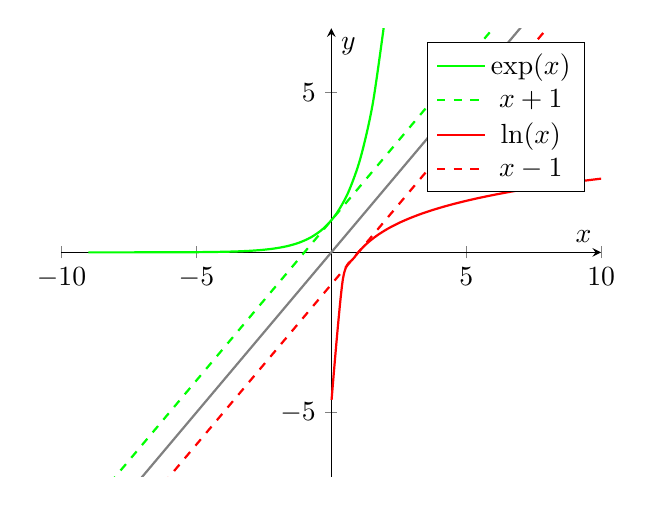
\begin{tikzpicture}
    \begin{axis}[
      axis lines=middle,
      xmin=-10,
      xmax=10,
      ymin=-7,
      ymax=7,
      xlabel={$x$},
      ylabel={$y$},
      legend pos=north east,
      ]

      \addplot[smooth,domain=-9:2,color=green,thick]{exp(x)};
      \addlegendentry{$\exp(x)$}
      \addplot[dashed,domain=-9:10,color=green,thick]{x+1};
      \addlegendentry{$x + 1$}

      \addplot[smooth,domain=0.01:10,color=red,thick]{ln(x)};
      \addlegendentry{$\ln(x)$}
      \addplot[dashed,domain=-9:10,color=red,thick]{x-1};
      \addlegendentry{$x - 1$}

      \addplot[smooth,domain=-9:10,color=gray,thick]{x};
    \end{axis}
    \end{tikzpicture}
  \end{center}

\end{Bemerkung}

\subsection{Die natürliche Zahl $e$}

\begin{Definition}
  \begin{itemize}
    \item $\exp(1) = \limn \left(1 +\dfrac{1}{n}\right)^n =: e$
    \item $\exp(-1) = \limn \left(1 -\dfrac{1}{n}\right)^n =: e^{-1}$
  \end{itemize}
  Wir nennen $e$ die Euler'sche Konstante, und benutzen diese als Basis des natürlichen Logarithmus.
  $$e = 2,71828182...$$
\end{Definition}

\begin{Theorem}
  \begin{itemize}
    \item $\exp(2) = \exp(1+1) = e^2$
    \item $\exp(3) = \exp(1+1+1) = e^3$
    \item $\exp(n) = ... = e^n \A \in \Z$
  \end{itemize}
  Allgemein: Für $x = \dfrac{q}{p}$ mit $p,q \in \Z, q \geq 1$ gilt:
  $$\exp(x) = \exp\left(\dfrac{p}{q}\right) = \exp\left(\dfrac{1}{q}+ ... + \dfrac{1}{q} \right) = \exp\left(\dfrac{1}{q}\right)^p = \sqrt[q]{e^p} = e^{p/q}$$
  $$\exp\left(\dfrac{1}{q}\right)^q = \exp\left(\dfrac{1}{q}+ ... + \dfrac{1}{q} \right) = \exp(1) = e$$
\end{Theorem}

\begin{Definition}
  Für $x \in \R$ schreiben wir: $e^x := \exp(x)$.
  \begin{itemize}
    \item $\exp(\log(2)) = 2$
    \item $\exp(2\log(2)) = 4$
    \item $\exp(n\log(2)) = 2^n$
    \item $2^x = \exp(x\log(2))$
  \end{itemize}
  Allgemeiner gilt: Für $a>0, x\in \R$:
  $$a^x = \exp(x\log(a))$$
  Daraus folgt, dass $a^x$ stetig ist, denn sie ist eine Verknüpfung stetiger Funktionen.
\end{Definition}

\begin{Bemerkung}
  Sei $x \in \R$, $a >0$
  $$a^x = \limn \sqrt[q_n]{a^{p_n}}$$
  für jede beliebige Folge $\left(\dfrac{p_n}{q_n}\right)_{n=0}^\infty$ in $\Q$ mit $\lim \dfrac{p_n}{q_n} = x$.\\
  Grund: $a^x$ ist stetig.
\end{Bemerkung}

\begin{Bemerkung}
  Wir verwenden $\log$, den natürlichen Logarithmus, auch geschrieben als $\ln$.
\end{Bemerkung}


\section{Grenzwerte von Funktionen}

Es sei $D \subseteq \R$ (Definitionsmenge) und $x_0 \in \R$. Angenommen $x_0 \in D$ oder $x_0$ ist ein Häufungspunkt von $D$.

\begin{Beispiel}[typisch]
  \begin{itemize}
    \item $D = (0,1)$ also: $x_0 \in [0,1]$
    \item $D = \left\{\dfrac{1}{n} \middle| n \geq 1, n\in \N \right\}$ also: $x_0 \in D$ oder $x_0 = 0$
    \item $D = \R^x = \R\backslash 0$ also $x_0 \in \R$
  \end{itemize}
\end{Beispiel}

\begin{Definition}[Grenzwert]
  Sei $D \subseteq \R$ (Definitionsmenge) und $x_0 \in \R$. Angenommen $x_0 \in D$ oder $x_0$ ist ein Häufungspunkt von $D$. Sei $f: D \to \R$ eine Funktion. Eine reelle Zahl $a$ heißt \textbf{Grenzwert von $f$ bei $x_0$} falls
  $$\A \varepsilon < 0 \E \delta > 0 : |x-x_0| < \delta \Rightarrow |f(x) - a| < \varepsilon$$
\end{Definition}

\begin{Beispiel}
  \begin{itemize}
    \item $D = (0,1), x_0 = 0$. $f: D\to\R, f(x) = x^2$. $a = \dfrac{1}{2}$ ist kein Grenzwert $a = 0$ ist es.
    \item $D = \R$ und $f(x) = sig(x)^2 = \left\{\begin{array}{c}
      1 \quad x \neq 0\\
      0 \quad x = 0
      \end{array}\right.$. $a = 1$ ist kein Grenzwert, denn für beispielsweise $\varepsilon = \dfrac{1}{3}$ gilt: $f(0) = 0$ aber $|f(0)-a| = 0 \not< \varepsilon$. $f$ hat keinen Grenzwert bei $x_0$
      \begin{Bemerkung}
         Durch die ältere Definition mit $x \neq x_0$, wäre auch bei $x_0 = 0$ ein Grenzwert obwohl $f$ nicht stetig ist. Wir verwenden allerdings die neue Definition. Die alte wird allerdings oftmals noch in der Literatur vorgefunden.
      \end{Bemerkung}
    \item $D = \R \backslash 0$, $f(x) = 1$ konstant. $x_0 = 0$ ist ein Häufungspunkt von $D$. Hier gilt: $a = 1$ ist Grenzwert von $f$ bei $x_0$.
  \end{itemize}
\end{Beispiel}

\begin{Bemerkung}
  Sei $D \subseteq \R$ (Definitionsmenge) und $x_0 \in \R$. Angenommen $x_0 \in D$ oder $x_0$ ist ein Häufungspunkt von $D$. Sei $f:D\to \R$. Falls es einen Grenzwert $a$ von $f$ bei $x_0$ gibt, dann ist dieser Grenzwert eindeutig bestimmt und wir schreiben:
  $$a = \lim \limits_{x \to x_0} f(x)$$
\end{Bemerkung}

\begin{Bemerkung}[Variante]
  Angenommen $x_0 \in D$. Betrachte die Einschränkung von $f$ auf $D \backslash \{x_0\}$, also $f^*:D\backslash\{x_0\} \to \R$. Schreibe
  $$\lim \limits_{\substack{x \to x_0 \\ x \neq x_0}} f(x) \text{ für } \limx f^*(x)$$
  falls dieser Grenzwert existiert.
\end{Bemerkung}

\begin{Bemerkung}
  \begin{Theorem}
    Sei $D\subseteq \R$, $x_0$ ein HP von $D$ und $x_0 \notin D$. Sei $f : D \to \R$. $a$ ist Grenzwert von $f$ bei $x_0$ genau dann wenn:
    $$\bar{f} : D \cup \{x_0\} \to \R, \bar{f}(x) = \left\{ \begin{array}{c}
      f(x) \quad x \in D\\
      a \quad x = x_0
    \end{array}\right.$$
    stetig bei $x_0$ ist.
  \end{Theorem}
  \begin{Beweis}
    Angenommen $a = \limx f(x)$ ist Grenzwert von $f$. Die Funktion $\bar{f}$ ist stetig bei $x_0$:
    $$\A \varepsilon < 0 \E \delta > 0 : |x-x_0| < \delta \Rightarrow |\bar{f}(x) - \bar{f}(x_0)| < \varepsilon \A x \in D \cup \{x_0\}$$
    $\Leftrightarrow \A \varepsilon < 0 \E \delta > 0 : |x-x_0| < \delta \Rightarrow |f(x) - a| < \varepsilon$, was der Definition der Stetigkeit von $f$ entspricht.
  \end{Beweis}
\end{Bemerkung}

\begin{Theorem}
  Sei $D \subseteq \R$ (Definitionsmenge) und $x_0 \in \R$. Folgende Aussagen sind äquivalent für $x_0 \in D$:
  \begin{enumerate}
    \item Die Funktion $f$ ist stetig bei $x_0$
    \item $\lim \limits_{\substack{x \to x_0 \\ x \neq x_0}} = f(x_0)$
    \item $\limx f(x) = f(x_0)$
    \item Für jede Folge $(y_n)_{n=0}\infty$ in $D$ mit Grenzwert $x_0 = \limn y_n$ gilt:
      $$\limn f(y_n) = f(x_0)$$
  \end{enumerate}
\end{Theorem}

\begin{Theorem}
  Seien $D,E \subseteq \R$, sei $f:D\to E$, so dass $\limx f(x) = a$ existiert und $a \in E$ gilt. Sei $g: E \to \R$ eine Funktion, die bei $a \in E$ stetig ist. Dann gilt:
  $$\limx g(f(x)) = g(a)$$
\end{Theorem}

\begin{Beweis}
  Sei $(z_n)_{n = 0}^\infty$ eine Folge in $D$ mit $\limn z_n = x_0$. Dann gilt:
  $$\limn f(z_n) = a \in E$$
  Die Funktion $g$ ist stetig bei $a \in E$, also konvergiert
  $$\limn g(f(z_n)) = g(a)$$
  nach dem Folgenkriterium für Stetigkeit.

  Also: Für jede Folge $(z_n)_{n = 0}^\infty$ in $D$ mit $\limn z_n = x_0$ gilt:
  $$\limn g(f(z_n)) = g(a)$$
  Also gilt
  $$\limx g(f(x)) = g(a)$$
\end{Beweis}

\begin{Beispiel}
  $D=(0,1)$, $f:D\to \R$ gegebenen durch $f(x) = \dfrac{1}{x(1-x)}$.

  Die Aussage $$\lim \limits_{x\to 2} f(x)$$ ist sinnlos.

  $\lim \limits_{x \to 0} f(x)$ existiert ebenfalls nicht. (es gibt keine reelle Zahl, die die Bedingung des Grenzwerts erfüllt.) Bzw. $ = \infty$
\end{Beispiel}

\subsection{Arten von Grenzwerten}

\begin{Definition}[Uneigentliche Grenzwerte]
  Wir schreiben
  $$\limx f(x) = \infty$$
  Für
  $$\A M \in \R \E \delta > 0 : |x-x_0| < \delta \Rightarrow f(x)> M \A x \in D$$
  Analog für $- \infty$
\end{Definition}

\begin{Beispiel}[diverse Grenzwerte]
  \begin{itemize}
    \item $D = \R, f: D \to \R, f(x) = x^3$\\
      $\lim \limits_{x \to 3} f(x) = f(3) = 27$ weil $f$ stetig stetig.\\
      $\lim \limits_{x \to \infty} f(x) = \infty$, denn $\A M \in \R \E R \in \R : x > R \Rightarrow f(x) > M \A x \in D$
    \item $D = \R, f: D \to \{-1,1\}, f(x) = sgn(x)$
      \begin{center}
        \begin{tikzpicture}
          \begin{axis}[
            domain=-4:4,
            axis x line = center,
            xmajorticks=false,
            axis y line = center,
            xlabel={$x$},
            ylabel={$y$},
          ]

            \addplot[thick,blue,domain=-4:0]{-1};
            \addlegendentry{$sgn(x)$}
            \addplot[thick,blue,domain=0:4]{1};
          \end{axis}
        \end{tikzpicture}
      \end{center}
      $$\lim \limits_{\substack{x \to 0 \\ x > 0}} = 1 \text{, der rechtsseitige Grenzwert}$$
    \item Alle weiteren Möglichkeiten siehe Skript, 6.4 Abbildung 6.110 (S. 150.)
  \end{itemize}
\end{Beispiel}

\begin{Definition}[Einseitiger Grenzwert]
  $$\lim \limits_{\substack{x \to x_0 \\ x > x_0}} = a$$
  bedeutet
  $$\A \varepsilon > 0 \E \delta > 0 : |x - x_0| < \delta \land x > x_0 \Rightarrow |f(x)-a|<\varepsilon \A x \in D$$
  Wir nennen dies den \textbf{rechtsseitigen Grenzwert} der Funktion.\\
  Analog definieren wir den linksseitigen Grenzwert.
\end{Definition}

\begin{Bemerkung}
  Der Fall mit $x \geq x_0$ ist ein anderer Fall! Dieser hatt möglicherweise eine andere Validität.
\end{Bemerkung}

\begin{Beispiel}
  Sei $f: \R_{> 0} \to \R$ mit $f(x) = x^x = \exp(x \log(x))$\\
  Existiert der Grenzwert $\lim \limits_{x \to 0} f(x)$?\\
  Berechne zuerst $\lim \limits_{y \to \infty} y \exp(-y) = \lim \limits_{y \to \infty} \dfrac{y}{\exp(y)}$.\\
  \textbf{Behauptung:}
  $$\lim \limits_{y \to \infty} y \exp(-y) = 0$$
  $$\Leftrightarrow \A \varepsilon > 0 \E R \in \R : y > R \Rightarrow |y \exp(-y)| < \varepsilon$$
  Es gilt: $\exp(z) = \limn \left( 1 +\dfrac{z}{n}\right)^n \geq \left( 1 +\dfrac{z}{2}\right)^2$ für $z > 0$.\\
  Folgt für $y > 0$ die Abschätzung
  $$0 \leq \dfrac{y}{\exp(y)} \leq \dfrac{y}{.\left(1+\dfrac{y}{2}\right)^2}$$
  Deshalb folgt wegen des Sandwich-Kriteriums
  $$0 \leq \lim \limits_{y \to \infty} \dfrac{y}{\exp(y)} \leq 0$$
  \textbf{Behauptung:} $\lim \limits_{x \to 0} x \log(x) = 0$.\\
  Sei $\varepsilon > 0$. Dann existiert ein $\delta > 0$ mit $y \exp(-y) < \varepsilon$ für alle $y > \dfrac{1}{\delta}$. Für $x \in \R_{> 0}$ mit $x < \exp\left(\dfrac{-1}{\delta}\right)$ gilt (Behauptung)
  $$|x \log(x)| < \varepsilon$$
  Setze $y = -\log(x)$. Dann gilt $y > \dfrac{1}{\delta}$ also $|y \exp(-y)| < \varepsilon$ also $|-\log(x)x| < \varepsilon$ (was zu zeigen war).\\
  $\exp : \R \to \R$ ist stetig bei $x_0 = 0$. Also:
  $$\lim \limits_{x \to 0} \exp(x \log(x)) = \exp(0) = 1$$
\end{Beispiel}

\subsection{Landau-Symbole}

Streng genommen handelt es sich nur um eine Notation.
\begin{Definition}[Landau-Symbole]
  Seien $D \subseteq \R$, $f,g :d \to \R$, $x_0 \in \R$ mit $x_0 \in D$ oder $x_0$ ist ein Häufungspunkt von $D$. (Auch $x_0 \in \{-\infty,\infty\}$). Wir schreiben
  \begin{itemize}
    \item $f(x) = \mathcal{O}(g(x))$ (großes Landau-O) für $x \to x_0$, falls $\delta >0$, $M > 0$ existieren mit
      $$|x - x_0| < \delta \Rightarrow |f(x)| \leq M |g(x)| \A x \in D$$
    \item $f(x) = \mathcal{O}(g(x))$ für $x \to -\infty$ bedeutet
      $$\E R \in \R,M > 0 : |f(x)| \leq M |g(x)| \text{ für } x \in D, x < R$$
      Für $+\infty$ würden sich die Beduingungen zu $x > R$ verändernn.
    \item $f(x) = o(g(x))$ (kleines Landau-o) für $x \to x_0$ bedeutet
      $$\A \varepsilon > 0 \E \delta > 0 : |f(x)| \leq \varepsilon |g(x)| \text{ für } x\in D \land |x - x_0| < \delta$$
      \begin{Theorem}
        Falls $g(x) \neq 0$ für $x \in D$ mit $|x - x_0| < \delta$, dann gilt:
        $$f(x) = o(g(x)) \text{ für } x \to x_0 \Leftrightarrow \limx \dfrac{f(x)}{g(x)} = 0$$
      \end{Theorem}
  \end{itemize}
\end{Definition}

\begin{Beispiel}
  \begin{itemize}
    \item $D = \R$, $x_0 = 0$, $f(x) = 1+x$, $g(x) = \exp(x)$.
    
    $|x| < \delta \Rightarrow |f(x)| < M |g(x)|$.
    
    Konkret: Für $|x| < 1$ gilt: $x+1 < 3 \exp(x)$
    
    Allgemein gilt: $1 + x = \mathcal{O}(\exp(x))$ für $x \to x_0$
    
    Aber auch: $1 + x + x^2= \mathcal{O}(\exp(x))$ für $x \to x_0$
    
    \begin{Bemerkung}
      Hier erkennt man die Gefahr dieser Notation: sie ist nicht eindeutig und das $=$ ist nicht wörtlich zu nehmen. (Es ist nicht transitiv.)
    \end{Bemerkung}
  \end{itemize}
\end{Beispiel}


\section{Normen und Konvergenz in Vektorräumen}

\begin{Bemerkung}
  Sei nachfolgend $K$ entweder der Körper $\R$ oder $\C$. Sei $V$ ein Vektorraum über $K$.
\end{Bemerkung}

\begin{Bemerkung}[Neue Definition der Exponentialfunktion]
  Bisherige Definition:
  $$\exp(x) := \limn \left(1 + \dfrac{x}{n}\right)^n$$
  Für $n \geq 1$ betrachte die stetige Funktion $f_n : \R \to \R$ mit $f_n(x) = \left(1 + \dfrac{x}{n}\right)^n$. Jetzt können wir definieren:
  $$\exp = \limn f_n$$
  Jetzt gilt
  $$\A x \in \R : \exp(x) = \limn f_n(x)$$
\end{Bemerkung}

\begin{Definition}[Norm]
  Eine \textbf{Norm} auf $V$ ist eine Abbildung $||.|| : V \to \R$ mit folgenden Eigenschaften.
  \begin{enumerate}
    \item Definitheit: $||v|| \geq 0 \A v \in V$ und
      $$||v|| = 0 \Leftrightarrow v = 0$$
    \item Homogenität:
      $$\A v \in V \A \alpha \in K : ||\alpha v|| = |\alpha| ||v||$$
    \item Dreiecksungleichung:
      $$||v+w|| \leq ||v|| + ||w||$$
  \end{enumerate}
  Wir nennen $(V, ||.||)$ einen normierten Vektorraum.
\end{Definition}

\begin{Beispiel}
  $V = K$. Dann ist der Betrag $|.| : V \to \R$ eine Norm.
\end{Beispiel}

\begin{Definition}[Induzierte Metrik]
  Sei $(V, ||.||)$ ein normierter Vektorraum. Die von $||.||$ \textbf{induzierte Metrik} auf $V$ ist:
  $$\begin{aligned}
    d : V\times V & \to \R \\
    v,w & \mapsto d(v,w) = ||v - w||
  \end{aligned}$$
\end{Definition}

\begin{Bemerkung}
  \begin{Theorem}
    Dieses $d$ ist tatsächlich eine Metrik.
  \end{Theorem}
  \begin{Beweis}
    \begin{itemize}
      \item Positive Definitheit:
        $$d(v,w) = ||v-w|| \geq 0 \A v,w \in V$$
        $$d(v,w) = 0 \Leftrightarrow ||v-w|| = 0 \Leftrightarrow v-w = 0 \Leftrightarrow v = w \text{ (Vektorraumaxiome)}$$
      \item Symmetrie:
        $$d(v,w) = ||v-w|| = |-1|||v-w|| = ||(-1)(v-w)|| = ||v-w|| = d(w,v)$$
      \item Dreiecksungleichung:\\
        Seien $v,w,z \in V$
        $$d(v,z) = ||v - z|| = ||v-w+w-z|| \leq ||v-w|| + ||w-z|| = d(v,w) + d(w,z)$$
    \end{itemize}
  \end{Beweis}
\end{Bemerkung}

\begin{Beispiel}
  $K = \R$, $V = \R^n$, $v = \left(\begin{array}{c}x_1\\...\\x_n \end{array}\right)$, $w = \left(\begin{array}{c}y_1\\...\\y_n \end{array}\right)$
  \begin{itemize}
    \item Setze für $v$:
      $$||v||_1 = \sum \limits_{i=1}^n |x_i| = |x_1| + |x_2| + ... + |x_n|$$
      Dann ist $||.||_1 : V \to \R$ eine Norm.
      \begin{Beweis}
        \begin{itemize}
          \item Positive Definitheit \checkmark
          \item Symmetrie \checkmark
          \item Dreiecksungleichung:
            Seien $v$ und $w$:
            $$||v+w||_1 = \sum |x_i + y_i| \leq \sum|x_i|+|y_i| = ||v||_1 + ||w||_1 \checkmark$$
        \end{itemize}
      \end{Beweis}
      Diese Norm auf $\R^n$ heißt \textbf{1-Norm}.

    \item Setze für $v$:
      $$||v_2|| = \sqrt{\sum \limits_{i=1}^n x_i^2}$$
      Auch $||.||_2 : \R^n \to \R$ ist eine Norm.
      \begin{Beweis}
        Beweis der Dreiecksungleichung ist mühsam und kann als Übung erfolgen.
      \end{Beweis}
      Diese Norm heißt \textbf{2-Norm}, sie wird auch als Euklidische Norm oder Standardnorm bezeichnet.

    \item Setze für $v$
      $$||v||_\infty = \max \{|x_1|,...,|x_n|\}$$
      Auch $||.||_\infty : \R^n \to \R$ ist eine Norm. Sie heißt \textbf{Maximumsnorm} oder $\infty$-Norm oder $\sup$-Norm.
  \end{itemize}
  \begin{Bemerkung}
    Die von $||.||_1$ induzierte Metrik ist die Manhattan-Metrik.
  \end{Bemerkung}

  \begin{Theorem}
    Allgemein kann man für eine reelle Zahl $p \geq 1$ schreiben:
    $$||v||_p = \sqrt[p]{\sum \limits_{i=1}^n |x_i|^p}$$
    Man kann zeigen: $||.||_p : \R^n \to \R$ eine Norm ist. Name: p-Norm.
  \end{Theorem}
\end{Beispiel}

\begin{Beispiel}
  Seien $a < b \in \R$. Sei $V = C([a,b])$ der Vektorraum aller stetigen Funktionen $f:[a,b]\to\R$.
  \begin{itemize}
    \item Für $f\in V$ setze:
      $$||f||_1 = \int_a^b |f(x)| dx$$
      Dann ist $||.||_1 : V \to \R$ eine Norm. Sie heißt 1-Norm oder $L^1$-Norm.
      \begin{Beweis}
        Definitiheit?\\
        Homogenität: folgt aus der Linearität des Integrals \checkmark\\
        Dreiecksungleichung: bereits bewiesen \checkmark
      \end{Beweis}

    \item Setze für $f \in V$
      $$||f||_2 = \sqrt{\int_a^b f(x)^2 dx}$$
      Dann ist $||.||_2 : V \to \R$ eine Norm. Sie heißt 2-Norm oder $L^2$-Norm.
      \begin{Beweis}
        Der Beweis der Dreiecksungleichung erfolgt später über einen allgemeinen Beweis.
      \end{Beweis}

    \item Setze für $f \in V$
      $$||f||_\infty = \max\{|f(x)| \mid x \in [a,b] \}$$
  \end{itemize}
  \begin{Theorem}
    Allgemein definiert
    $$||f||_p = \sqrt[p]{\int_a^b |f(x)|^p dx}$$
    eine Norme auf $V$, gennant p-Norm oder $L^p$-Norm.
  \end{Theorem}
\end{Beispiel}

\begin{Bemerkung}
  $L^x$-Normen stehen für \textbf{Lebesgue Normen}, erdacht von Henry Lebesgue.
\end{Bemerkung}

\begin{Definition}
  Sei $V$ ein $K$-Vektorraum. Seien $||.||_1$ und $||.||_2$ Normen auf $V$. Wir sagen $||.||_1$ und $||.||_2$ sind \textbf{äquivalent}, falls $\E A, B \in \R_{>0}$ mit:
  \begin{itemize}
    \item $||v||_1 \leq A ||v||_2$
    \item $||v||_2 \leq B ||v||_1$
  \end{itemize}
  für alle $v \in V$ existiert.
\end{Definition}

\begin{Bemerkung}
  Sobald $V$ ein nicht-trivialer Vektorraum ist, ergibt sich wegen der Definitheit der Norm, dass $A,B > 0$ sind.
\end{Bemerkung}

\begin{Beispiel}
  \begin{itemize}
    \item Auf $\R^n = V$ betrachte:
      \begin{itemize}
        \item $||v||_1 = \sum \limits_{i = 1}^n |x_i|$
        \item $||v||_\infty = \max \{|x_1|,...,|x_n|\}$
      \end{itemize}
      In jedem Fall gilt: $||v||_\infty \leq 1 ||v||_1$. Außerdem erkennt man: $||v||_1 \leq n ||v||_\infty$
      \begin{Bemerkung}
        Wir werden sehen, dass auf dem $\R^n$ alle Normen äquivalent sind.
      \end{Bemerkung}
    \item Auf $V = \mathcal{C}([a,b])$ betrachte:
      \begin{itemize}
        \item $||f||_1 = \int_a^b |f(x)|dx$ mit $f \in V$
        \item $||f||_\infty = \max\{|f(x)| \mid x \in [a,b]\}$
      \end{itemize}
      Es gilt: (optimistischerweise)
      $$\begin{aligned}
        ||f||_1 \leq (b-a) ||f||_\infty \\
        ||f||_\infty \leq {\color{red}?}||f||_1
      \end{aligned}$$
      Vermutung: Nicht konstruierbar. Beweis erfolgt in Kürze.
  \end{itemize}
\end{Beispiel}

\begin{Theorem}
  Sei $V$ ein $K$-Vektorraum, seien $||.||_1$ und $||.||_2$ Normen auf $V$. Dann sind folgende Aussagen äquivalent: (TFAE)
  \begin{enumerate}
    \item $||.||_1$ und $||.||_2$ sind äquivalent.
    \item Die Identitätsabbildung $V_{||.||_1} \to V_{||.||_2}$ ist stetig, und genauso $V_{||.||_2} \to V_{||.||_1}$.
    \item Eine Teilmenge $U \subseteq V$ ist offen bezüglich der von $||.||_1$ induzierten Metrik genau dann, wenn sie oggen bezüglich der von $||.||_2$ induzierten Metrik ist.
    \item Eine Folge $(v_n)_{n=0}^\infty$ in $V$ konvergiert nach $w \in V$ bezüglich $||.||_1$ genau dann, wenn $V_N$ gegen $w$ bezüglich $||.||_2$ konvergiert.
      \begin{Bemerkung}
        Dies ist besonders nützlich bei Grenzwertbestimmung. Man kann einen Grenzwert über eine beliebige äquivalente Norm berechnen, also insbesondere der, die bei der Rechnung am besten passt.
      \end{Bemerkung}
  \end{enumerate}
\end{Theorem}

\begin{Beweis}
  \begin{itemize}
    \item $2 \Leftrightarrow 3$ entspricht der topologischen Charakterisierung von Stetigkeit.
    \item $2 \Leftrightarrow 4$ Folgenkriterium für Stetigkeit.
    \item $1 \Rightarrow 4$ Sei $A \in \R_{> 0}$ mit $||v||_1 \leq A ||v||_2$. Sei $(v_n)_{n=0}^\infty$ eine Folge in $V$, die bezüglich $||v||_2$ gegen $w \in V$ konvergiert.\\
      Sei $\varepsilon > 0$. $\E N \in \N$ mit:
      $$\begin{aligned}
        n \geq N &\Rightarrow ||v_n - w||_2 < \varepsilon \dfrac{1}{A}\\
        &\Leftrightarrow A ||v_n - w||_2 < \varepsilon\\
        &\Rightarrow ||v_n - w||_1 < \varepsilon
      \end{aligned}$$
      Diese Aussage können wir auch anders herum für $B$ zeigen. Damit haben wir insgesamt aber nur die Hinrichtung.
    \item $3 \Rightarrow 1$ Betrachte $U = \{v \in V \mid ||v||_2 < 1 \} = B(0,1)$ bezüglich $||.||_2$.\\
      Die Menge $U$ ist offen bezüglich beider Normen. Insbesondere gilt $0 \in U$.\\
      $$\E \delta > 0 : \{v\in V \mid ||v||_1 < \delta \} \subseteq U =\{v\in V \mid ||v||_2 < 1\}$$
      Also kann man sagen:
      $$\begin{aligned}
        ||v||_1 < \delta &\Rightarrow ||v||_2 < 1 \A v \in V \\
        ||v||_1 &\leq ||v||_2 \dfrac{1}{\delta} (= A)
      \end{aligned}$$
      In die andere Richtung erhalten wir wieder $B$.\\
      Sei $v \in V$, $v \neq 0$, $v = \alpha w$ für:
      $$\alpha = \dfrac{||v||_1}{\delta} \qquad w = \dfrac{\delta}{||v||_1} v \qquad ||w||_1 \leq \delta$$
      $\Rightarrow$ (Hypothese) $||w||_2 \leq 1$

      $||v||_2 = ||\alpha w||_2 = \alpha ||w||_2 \leq \alpha = \dfrac{||v||_1}{\delta}$
  \end{itemize}
\end{Beweis}

Zurück zum obigen Beispiel:
\begin{Beispiel}
  Wir wollen zeigen, dass beide Normen nicht äquivalent sind, also beispielsweise, dass Folgen existieren, die für eine Norm konvergieren, aber für die andere nicht.\\
  Betrachte: $(f_n)_{n=0}^\infty$ die Folge in $V = \mathcal{C}([0,1])$ siehe Foto oder: (fn linear wachsend bis $2^{-n}$ und ab dann konstant 1). Sei $g:[0,1] \to \R$ konstant mit Wert $1$.s\\
  Behauptung:
  $$\limn f_n = g \text{ bezüglich } ||.||_1$$
  \begin{Beweis}
    $$||f_n - g||_1 = \int_0^1 |f_n - g| dx = 2^{-(n+1)}$$
  \end{Beweis}
  aber es gilt:
  $$||f_n - g||_\infty = 1 \A n$$
  Also konvergiert $f_n$ nicht gegen $g$.\\
  $\Rightarrow ||.||_1$ und $||.||_\infty$ sind nicht äquivalent.
\end{Beispiel}

\subsection{Skalare Normen}

\begin{Definition}[Skalarprodukt]
  Sei $V$ ein $K$-Vektorraum. \textbf{Ein} Skalarprodukt auf $V$ ist eine Abbildung
  $$\begin{aligned}
    V \times V &\to K \\
    (v,w) &\mapsto <v,w>
  \end{aligned}$$
  mit folgenden Eigenschaften:
  \begin{enumerate}
    \item Sesquilinearität: $\A \alpha,\beta \in K, v_1,v_2,w_1,w_2,w,v$ gilt:
      $$<\alpha v_1 + \beta v_2 , w> = \alpha<v_1,w> + \beta<v_2,w>$$
      $$<v,\alpha w_1 + \beta w_2> = \overline{\alpha}<v,w_1> + \overline{\beta}<v,w_2>$$
      Für $K = \C$. Für $\R$ ist die komplexe Konjugation überflüssig.
    \item Symmetrie: $<v,w> = \overline{<w,v>}$
    \item Definitheit (insbesondere positive Definitiheit): $\A v \in V:$
      $$<v,v> \in \R_{\geq 0} \text{ und } <v,v> = 0 \Leftrightarrow v = 0$$
  \end{enumerate}
\end{Definition}

\begin{Beispiel}
  $V= \mathcal{C}([a,b])$, $<f,g> = \int_a^b f(x)\overline{g(x)} dx$\\
  Linearität, Symmetrie \checkmark.\\
  Definitheit: $<f,f> = \int_a^b|f(x)|^2 dx$ Konsequenzen sind die der Definitheit.\\
  \begin{Theorem}
    $$||f||_2 = \sqrt{<f,f>}$$
  \end{Theorem}
\end{Beispiel}

\begin{Theorem}[Cauchy-Schwarz]
  Sei $V$ ein $K$-Vektorraum, $<.,.>$ ein Skalarprodukt auf $V$. Für $v \in V$ schreibe $||v|| = \sqrt{<v,v>}$.\\
  Dann gilt:
  $$|<v,w>| \leq ||v||\cdot ||w|| \A v,w \in V$$
\end{Theorem}

\begin{Beweis}
  ObdA $v \neq 0, w \neq 0$.\\
  Setze $\alpha = <v,w> \dfrac{1}{||w||^2}$
  $$\begin{aligned}
    0 \leq ||v - \alpha w||^2 &= <v-\alpha w, v-\alpha w>\\
    &= <v,v> - \alpha <w,v> - \overline{\alpha}<v,w>+ \alpha \overline{\alpha}<w,w>\\
    &= ||v||^2 - 2 \dfrac{|<v,w>|^2}{||w||^2} + \dfrac{|<v,w>|^2}{||w||^4} ||w||^2
  \end{aligned}$$
  Folgt:
  $$||v||^2 \geq \dfrac{|<v,w>|^2}{||w||^2}$$
\end{Beweis}

\begin{Bemerkung}
  Diese Relation ist eine Gleichheit $\Leftrightarrow$ $v$,$w$ kollinear (also $v = \alpha w $)
\end{Bemerkung}

\begin{Theorem}
  Sei $V$ ein $K$-Vektorraum, $<.,.>$ ein Skalarprodukt auf $V$. Dann definiert die Funktion
  $$v \mapsto ||v|| := \sqrt{<v,v>}$$
  eine Norm auf $V$.
\end{Theorem}

\begin{Beweis}
  Same procedure as last time, Miss Sophie? Same procedure as \textbf{every} time, James! Definitheit, Homogenität, Dreiecksungleichung.
  \begin{itemize}
    \item $||v|| = 0 \Leftrightarrow \sqrt{<v,v>} = 0 \Leftrightarrow <v,v> = 0 \Leftrightarrow = 0$
    \item Seien $\alpha \in K$, $v \in V$
      $$\begin{aligned}
        ||\alpha v || &= \sqrt{<\alpha v, \alpha v>}\\
        &= \sqrt{\alpha\overline{\alpha} <v,v> }\\
        &= \sqrt{|\alpha|^2 <v,v> }\\
        &= |\alpha| \cdot ||v||
      \end{aligned}$$
    \item Seien $v,w \in V$.
      $$\begin{aligned}
        ||v + w||^2 &= <v+w ,v+w>\\
        &= ||v||^2 + <v,w> + <w+v> + ||w||^2\\
        &= ||v||^2 + 2 Re(<v,w>) + ||w||^2 \text{ denn vw und wv sind komplex konjugiert}\\
        &\leq ||v||^2 + 2 |<v,w>| + ||w||^2\\
        &\leq ||v||^2 + 2 ||v||\cdot||w|| + ||w||^2 \text{ diese Umformung erfolgt über CS}\\
        &= (||v||+||w||)^2
      \end{aligned}$$
      $$\Rightarrow ||v+w|| \leq ||v|| + ||w||$$
  \end{itemize}
\end{Beweis}

\begin{Beispiel}[Anwendung]
  $$V = \mathcal{C}([a,b]), ||f||_2 = \sqrt{\int_a^b f(x)^2 dx}$$
  $||f||_2$ definiert also eine Norm auf $V$. Grund:
  $$<f,g> = \int_a^b f(x)\overline{g(x)} dx$$
  definiert ein Skalarprodukt.
\end{Beispiel}

\begin{Theorem}
  Sei $V = K^d$, $d \geq 0$.

  Eine Folge $(v_n)_{n=0}^\infty$ konvergiert bezüglich der 1-Norm $\Leftrightarrow$ sie konvergiert koordinatenweise.
\end{Theorem}

\begin{Beweis}
  Schreibe $π_j : V \to K$ für die lineare Abbildung $π_j(v) = x_j, v = \left(\begin{array}{c}x_1 \\ ... \\ x_j\end{array}\right)$.\\
  $(v_n)_{n=0}^\infty$ konvergiert koordinatenweise $\Leftrightarrow (π_j (v_n))_{n=0}^\infty$ konvergiert für alle $1 \leq j \leq d$\\
  Angenommen $(v_n)_{n=0}^\infty$ konvergiert nach $w \in V$
  $$\Leftrightarrow \A \varepsilon > 0 \E N \in \N : ||v_n - w|| < \varepsilon \A n \geq N$$
  $$\Leftrightarrow \A \varepsilon > 0 \E N \in \N : \sum \limits_{j = 1}^d |π_j(v_n - w)| < \varepsilon \A n \geq N$$
  $$\Rightarrow \A \varepsilon > 0 \E N \in \N : |π_j(v_n) - π_j (w)| < \varepsilon \A n \geq N$$
  $$\Rightarrow (π_j (v_n))_{n=0}^\infty \text{ konvergiert gegen } π_j(w)$$
  Angenommen $(π_j(v_n))_{n=0}^\infty$ konvergiert gegen $w_j$ für $j = 1,2, ..., d$. Setze $w = \left(\begin{array}{c}w_1 \\ ... \\ w_d\end{array}\right)$ also $π_j(w) = w_j$
  $$\A \varepsilon > 0 \E N : |π_j(v_n) - π_j (w)| < \varepsilon \dfrac{1}{d}\A n \geq N$$
  $$\A \varepsilon > 0 \E N : ||v_n - w||_1 < d \varepsilon \dfrac{1}{d} = \varepsilon \A n \geq N$$
\end{Beweis}

\begin{Theorem}[Heine-Borel]
  Sei $(v_n)_{n=0}^\infty$ eine bezüglich der 1-Norm beschränkte Folge in $K^d$. Dann besitzt $(v_n)_{n=0}^\infty$ eine bezüglich der 1-Norm konvergente Unterfolge, also eine Häufungspunkt.
\end{Theorem}

\begin{Bemerkung}
  Wir erweitern dies in Kürze auf beliebige Normen.
\end{Bemerkung}

\begin{Beweis}
  Sei $(v_n)_{n=0}^\infty$ beschränkt. Dann ist $(π_j(v_n))_{n=0}^\infty$ eine beschränkte Folge in $K$. Ersetze $(v_n)_{n=0}^\infty$ durch eine Unterfolge, so dass $(π_j(v_n))_{n=0}^\infty$ weiterhin konvergiert. Selbes für $π_2, π_3 ...$. Dies entspricht einer Unterfolge, die koordinatenweise koordinatenweise konvergiert.

  $\Rightarrow$ es handelt sich um eine konvergente Unterfolge.
\end{Beweis}

\begin{Theorem}
  Sei $V$ ein endlichdimensionaler $K$-Vektorraum. Alle Normen auf $V$ sind zueinander äquivalent.
\end{Theorem}

\begin{Beweis}
  Vorbemerkung: Ist $(V,||.||)$ ein normierter Vektorraum, so ist $||.||:V \to \R$ stetig.\\
  Grund: Für $v_0 \in V$ gilt:
  $$||v-v_0|| < \varepsilon \Rightarrow | ||v||-||v_0||| < \varepsilon = \delta$$
  Sei $V$ endlichdimensional, $e_1,..., e_d$ eine Basis von $V$. Sei $||.||$ eine beliebige Norm auf $V$.\\
  Setze
  $$||v||_1 = \sum \limits_{i=1}^d|x_i| \text{ für } v = x_1 e_1 + ... + x_d e_d$$
  Das definiert eine Norm auf $V$.\\
  Behauptung: $\E A,B$ mit:
  $$||v|| \leq A ||v||_1$$
  $$||v||_1 \leq B ||v||$$
  Für $v = x_1 e_1 + ... + x_d e_d$ gilt
  $$\begin{aligned}
    ||v|| = \left|\left| \sum \limits_{i=1}^d x_i e_i \right|\right| &\leq \sum \limits_{i=1}^d |x_i| ||e_i||\\
    &\leq \left( \sum \limits_{i=1}^d |x_i|\right) \cdot \underbrace{\max\{||e_1||,...,||e_d||\}}_{A}\\
    &= A ||v||_1
  \end{aligned}$$
  Setze $$S = \{v \in V \mid ||v||_1 = 1\} \text{ und } \delta = \inf\{||v|| \mid v \in S\}$$
  Sei $(v_n)_{n=0}^\infty$ eine Folge in $S$ mit
  $$\limn ||v_n|| = \delta$$
  Die Folge $(v_n)_{n=0}^\infty$ ist $||.||_1$-beschränkt. Heine-Borel besagt also, dass eine konvergente Teilfolge existiert.

  Ersetze $(v_n)_{n=0}^\infty$ durch eine solche Teilfolge.
  $$w = \limn v_n \text{ (bezüglich $||.||_1$)} \quad \delta = \limn ||v_n|| \text{ in } \R$$
  $$\A \varepsilon > 0 \E N \in \N : n \geq N \Rightarrow ||v_n - w||_1 < \dfrac{\varepsilon}{A} \Rightarrow ||v_n - w|| < \varepsilon$$
  $$w = \limn v_n \text{ bezüglich } ||.||$$
  Nach Vorbemerkung gilt:
  $$||w|| = \limn ||v_n|| = \delta \text{ in } \R$$
  $$||w||_1 = \limn ||v_n||_1 = 1$$
  Also $w = \limn v_n$ bezüglich $||.||_1$

  Folgt:
  $$||w||_1 \neq 0 \Rightarrow w \neq 0 \Rightarrow ||w|| \neq 0 \Rightarrow \delta > 0$$
  Sei $B := \frac{1}{\delta}$

  Für $v\in V, v\neq 0$ gilt:
  $$\dfrac{1}{||v||_1} v \in S$$
  also
  $$0 < \delta \leq \left|\left| \dfrac{1}{||v||_1} v \right|\right| = \dfrac{||v||}{||v||_1} \Rightarrow ||v||_1 \leq B ||v|| \A v \in V$$
\end{Beweis}

\begin{Korollar}
  jede beschränkte Folge in einem endlichdimensionalen $K$-Vektorraum besitzt eine konvergente Unterfolge (bezüglich einer beliebigen Norm).
\end{Korollar}

\begin{Korollar}
  Sei $V$ eine endlichdimensionaler $K$-Vektorraum. Jede Cauchy-Folge in $V$ konvergiert (bezüglich einer beliebigen Norm).

  Oder auch: $(V,||.||)$ ist vollständig.
\end{Korollar}

\begin{Bemerkung}
  Prähilbertraum (Vektorraum + Skalarprodukt) + Vollständigkeit = Hilbert-Raum


  Normierter Vektorraum + Vollständigkeit = Banach-Raum
\end{Bemerkung}

\end{document}
